\documentclass[a4paper,oneside,12pt]{extarticle}

\usepackage[utf8]{inputenc}
\usepackage[english]{babel}
\usepackage{amssymb,amsthm,mathtools,enumitem,geometry,hyperref,booktabs}
\usepackage{graphicx}
\usepackage{xcolor}
\usepackage{tikz}
\usetikzlibrary{calc,patterns,decorations.pathreplacing}
\usepackage{tikz-cd}
\usepackage{pgfplots}
\usepgfplotslibrary{fillbetween}
\pgfplotsset{compat=1.18}
\usepackage{float}
\usepackage{placeins}

\geometry{lmargin=15mm,rmargin=15mm,tmargin=10mm,bmargin=10mm,includeheadfoot}
\pagestyle{plain}
\frenchspacing

\theoremstyle{plain}
\newtheorem{proposition}{Proposition}
\newtheorem{lemma}[proposition]{Lemma}

\theoremstyle{definition}
\newtheorem{definition}[proposition]{Definition}
\newtheorem{example}[proposition]{Example}

\theoremstyle{remark}
\newtheorem{remark}[proposition]{Remark}

\newcommand*{\E}{\mathbb{E}}
\newcommand*{\Var}{\mathrm{Var}}
\newcommand*{\mP}{\mathbb{P}}
\newcommand*{\mR}{\mathbb{R}}
\newcommand*{\mbF}{\mathcal{F}}
\newcommand*{\ve}{\varepsilon}

\begin{document}
\begin{titlepage}
\begin{center}

{\footnotesize\scshape\color{gray}
Working Notes in Quantitative Risk and Modeling
}

\vfill

{\LARGE\bfseries Homoscedasticity and Its Testing:\\[4pt]
From Conditional Expectation to the Breusch--Pagan Test}

\vspace{36pt}

{\normalsize Boris Garbuzov}

\vfill

{\Large\bfseries Part~12~/~12}

\vspace{6pt}

{\Large\bfseries The Breusch--Pagan Test:\\Likelihood Foundations and Score Analysis}

\vfill

{\small July 2026}

\end{center}
\end{titlepage}

\setcounter{section}{0}
\setcounter{tocdepth}{2}
\tableofcontents
\newpage

\section{The Breusch--Pagan Test: Likelihood Foundations and Score Analysis}
\label{sec:bp-likelihood}

\subsection{Where the likelihood comes from}
\label{subsec:likelihood}

We follow Boris's notes of July~5, 2026 (note~58).

\subsubsection*{The question}

Boris interrupted the Probabilist's exposition of the score and asked: where
does the likelihood come from in the first place?  The Probabilist proposed
defining the likelihood through $\varepsilon$.  Boris objected:
if $\varepsilon \sim \mathcal{N}(0,1)$ and its distribution does
not depend on $\beta$, then $\beta$ will not appear in the
likelihood.  The Probabilist replied: the distribution of $\varepsilon$ does
not depend on $\beta$, but the \emph{observed value} of $\varepsilon$
does.  This distinction is the key.

\subsubsection*{The model}

We work in the simplest case: $p = 1$, $z = x$, intercept absorbed.
The full model is
\begin{align*}
  Y &= \beta_0 + \beta_1 X + U, \\
  U &= \sqrt{h(\alpha_0 + \alpha_1 X)}\cdot\varepsilon, \\
  \varepsilon &\perp X, \quad \varepsilon \sim \mathcal{N}(0,1).
\end{align*}
Introducing the shorthand $\sigma_x^2 := h(\alpha_0 + \alpha_1 x)$,
this becomes
\[
  Y = \beta_0 + \beta_1 X + \sigma_X \cdot \varepsilon.
\]
What is given (observed): $X, Y$.  What is deterministic and unknown:
$\beta_0,\beta_1,\alpha_0,\alpha_1$ (and $h$, treated as known in BP).
What is random and unobserved: $U$, $\varepsilon$, and — in the
random-regressor framework — $X$ itself.  The distribution of $X$
is a nuisance: it factors out of the conditional likelihood.

\subsubsection*{Expressing $\varepsilon$ through observables}

Inverting the model for $\varepsilon$:
\[
  \varepsilon
  \;=\; \frac{Y - \beta_0 - \beta_1 X}{\sqrt{h(\alpha_0 + \alpha_1 X)}}
  \;=\; \frac{Y - \beta_0 - \beta_1 X}{\sigma_X}.
\]
This expression is not observed directly — it depends on the data
$(X, Y)$ \emph{and} on the parameters $(\beta, \alpha)$.  Call it
$\varepsilon(y, x;\beta,\alpha)$ to make the dependence explicit.
For the $i$-th observation:
\[
  \varepsilon_i(\beta,\alpha)
  \;:=\;
  \frac{y_i - \beta_0 - \beta_1 x_i}{\sigma_{x_i}},
  \qquad
  \sigma_{x_i}^2 = h(\alpha_0 + \alpha_1 x_i).
\]

\subsubsection*{Why $\beta$ participates in the likelihood}

Boris's worry was: $\varepsilon \sim \mathcal{N}(0,1)$ with no
parameters in its distribution, so $\beta$ cannot appear.  The
resolution: the distribution of $\varepsilon$ is parameter-free, but
the \emph{value} it takes at observation $i$ is $\varepsilon_i(\beta,
\alpha)$, which depends on $\beta$.  The likelihood is the density of
the observed data evaluated at the observed values — and the
transformation from $(y_i, x_i)$ to $(\varepsilon_i, x_i)$ has a
Jacobian.

Concretely: since $\varepsilon_i = (y_i - \beta_0 - \beta_1 x_i)/
\sigma_{x_i}$, the map $y_i \mapsto \varepsilon_i$ has Jacobian
$\partial\varepsilon_i/\partial y_i = 1/\sigma_{x_i}$.
By the change-of-variables formula, the density of $Y_i$ given
$X_i = x_i$ is
\[
  p(y_i \mid x_i;\,\beta,\alpha)
  \;=\;
  \phi\!\left(\varepsilon_i(\beta,\alpha)\right)
  \cdot
  \frac{1}{\sigma_{x_i}},
\]
where $\phi$ is the standard normal density.  Writing this out:
\[
  p(y_i \mid x_i;\,\beta,\alpha)
  \;=\;
  \frac{1}{\sqrt{2\pi}\,\sigma_{x_i}}
  \exp\!\left(-\frac{(y_i - \beta_0 - \beta_1 x_i)^2}{2\sigma_{x_i}^2}\right).
\]
The log-likelihood for the full sample (conditioning on the $x_i$) is:
\[
  \boxed{
  l(\beta,\alpha)
  \;=\;
  -\frac{n}{2}\log(2\pi)
  \;-\; \frac{1}{2}\sum_{i=1}^n \log\sigma_{x_i}^2
  \;-\; \frac{1}{2}\sum_{i=1}^n
  \frac{(y_i - \beta_0 - \beta_1 x_i)^2}{\sigma_{x_i}^2}.
  }
\]
Both $\beta$ and $\alpha$ appear: $\beta$ through the residual
$y_i - \beta_0 - \beta_1 x_i$ in the last sum, and $\alpha$ through
$\sigma_{x_i}^2 = h(\alpha_0 + \alpha_1 x_i)$ in both the second
and third terms.  This is exactly the log-likelihood used in the
BP paper (their formula before the Theorem).

\begin{remark}[The measure of $X$ is a nuisance that drops out]
In the random-regressor framework, the joint density of $(Y_i, X_i)$
factorises as $p(y_i, x_i) = p(y_i|x_i;\beta,\alpha)\cdot p_X(x_i)$.
The log-likelihood for the full sample is therefore
\[
  \sum_i \log p(y_i|x_i;\beta,\alpha) + \sum_i \log p_X(x_i).
\]
The second sum does not depend on $(\beta,\alpha)$, so it is
irrelevant for any inference about those parameters.  The distribution
of $X$ is a nuisance — it is never specified, and the likelihood
analysis proceeds entirely through the conditional piece $p(y|x;\beta,
\alpha)$.  This is why neither BP nor Koenker say anything about the
distribution of $X$.
\end{remark}

\subsubsection*{The mixed terminology Boris identifies}

Boris observes that the model as written combines elements from two
papers.  Let us be precise.

\textbf{From BP (1979):} The parametrisation $\sigma_t^2 = h(z_t'\alpha)$
with $h$ a twice-differentiable positive function, and the direct
distributional assumption $u_t \mid x_t \sim \mathcal{N}(0,\sigma_t^2)$.
BP have no $\varepsilon$ in their paper: the Gaussian property sits on
$u$ itself, not on a standardised quantity.
The log-likelihood above is BP's likelihood verbatim.

\textbf{From Koenker (1981):} The product structure $u_i = \sigma_i
\varepsilon_i$ where $\varepsilon_i$ are i.i.d.\ from an
\emph{unspecified} distribution $F$ with mean zero, variance $\sigma^2$,
and finite fourth moment.  $F$ is \textbf{not} required to be Gaussian
--- this is Koenker's central generalisation.  When $F$ is Gaussian,
Koenker's model coincides with BP's; when $F$ is non-Gaussian, the
BP test statistic has incorrect size (Koenker's main result).

\textbf{The mixed model Boris writes} uses the product form
$U = \sigma_X \varepsilon$ with $\varepsilon \sim \mathcal{N}(0,1)$
and $\sigma_X^2 = h(\alpha_0 + \alpha_1 X)$.  This is \emph{BP's model
rewritten in product notation} --- it is not Koenker's model.
Koenker's model replaces $\varepsilon \sim \mathcal{N}(0,1)$ with
$\varepsilon \sim F$ (non-Gaussian).

\begin{remark}[Correction to note~58]
The Probabilist points out that in note~58 the Gaussian property was attributed
incorrectly.  The corrected picture: BP specify $u$ as conditionally
Gaussian directly, with no $\varepsilon$; Koenker introduces $\varepsilon$
precisely to drop the Gaussian assumption.  Writing the mixed model with
$\varepsilon \sim \mathcal{N}(0,1)$ recovers BP, not Koenker.
\end{remark}

\begin{remark}[Summary of parameters and their roles]
\begin{center}
\small
\begin{tabular}{lll}
\toprule
Object & Random or deterministic & Observed? \\
\midrule
$X_i, Y_i$ & Random (in RR framework) & Yes \\
$U_i, \varepsilon_i$ & Random & No \\
$\sigma_{X_i}$ & Random (function of $X_i$) & No \\
$\beta_0, \beta_1$ & Deterministic, unknown & No \\
$\alpha_0, \alpha_1$ & Deterministic, unknown & No \\
$h(\cdot)$ & Deterministic, known & --- \\
Distribution of $X$ & --- (nuisance) & Irrelevant for $l$ \\
\bottomrule
\end{tabular}
\end{center}
The likelihood $l(\beta,\alpha)$ depends on both parameter vectors:
$\beta$ through the residuals, $\alpha$ through the scale function.
\end{remark}

%--------------------------------------------------------------------

\subsection{Likelihood of a pivot}
\label{subsec:pivot-likelihood}

We follow Boris's notes of July~7, 2026 (note~59).

\subsubsection*{Warm-up: the location-normal family}

Before tackling the BP model, consider the simplest possible case.
Let $X \sim \mathcal{N}(\mu, 1)$ with $\mu \in \mathbb{R}$ unknown
and variance fixed at~$1$.  We observe a single value~$x$.

The \textbf{pivot} is
\[
  Z \;=\; X - \mu.
\]
Its distribution is $\mathcal{N}(0,1)$ for every value of $\mu$ —
fixed, no parameters.  The density of $Z$ is
\[
  \phi(z) \;=\; \frac{1}{\sqrt{2\pi}}\,e^{-z^2/2},
\]
a completely parameter-free function.

Now form the likelihood of $\mu$ given the observed $x$.  The
Jacobian of the map $x \mapsto z = x - \mu$ is $\partial z/\partial
x = 1$ — a pure shift has no scale change.  Therefore:
\[
  L(\mu \mid x)
  \;=\; \phi(x - \mu) \cdot 1
  \;=\; \frac{1}{\sqrt{2\pi}}\,\exp\!\left(-\frac{(x-\mu)^2}{2}\right).
\]
The log-likelihood is $l(\mu) = \mathrm{const} - \frac{1}{2}(x-\mu)^2$,
maximised at $\hat\mu = x$.

\medskip
Let us make Boris's observation precise in this simple case.

\textbf{The distribution of $Z$ does not depend on $\mu$} — true: $Z
\sim \mathcal{N}(0,1)$ always.

\textbf{But $Z$ still appears in the argument of the density} — the
observed value of the pivot is $z = x - \mu$, which depends on $\mu$.
When we evaluate the density at the observed value, we get
$\phi(x-\mu)$, which is not constant.

\textbf{One function does the work} — in the location family the
Jacobian is trivially 1, so there is only one source of
parameter-dependence: the argument $x - \mu$ of $\phi$.  The
``compensation'' Boris describes is: as $\mu$ varies, the function
$x \mapsto x - \mu$ shifts, and this shift is exactly what keeps the
distribution of $Z$ fixed.  But for the likelihood we hold $x$ fixed
and vary $\mu$ — the shift no longer compensates, and the
parameter-dependence in the argument is exposed.

\begin{example}
Take $x = 3$.  Then:
\begin{center}
\small
\begin{tabular}{cccc}
\toprule
$\mu$ & $z = x - \mu$ & $\phi(z)$ & $L(\mu)$ \\
\midrule
$0$ & $3.0$ & $0.0044$ & $0.0044$ \\
$1$ & $2.0$ & $0.054$ & $0.054$ \\
$2$ & $1.0$ & $0.242$ & $0.242$ \\
$3$ & $0.0$ & $0.399$ & $0.399$ \\
$4$ & $-1.0$ & $0.242$ & $0.242$ \\
$5$ & $-2.0$ & $0.054$ & $0.054$ \\
\bottomrule
\end{tabular}
\end{center}
The likelihood peaks at $\hat\mu = x = 3$, where the pivot value
is $z = 0$ (the mode of $\phi$).  At every row, $z = x-\mu$ is a
different number — the distribution of $Z$ is always $\mathcal{N}(0,1)$,
but which \emph{value} we sit at in that distribution changes.
\end{example}

\begin{remark}[For $n$ i.i.d.\ observations]
With $x_1,\ldots,x_n$ i.i.d.\ $\mathcal{N}(\mu,1)$, the pivots are
$z_i = x_i - \mu$, all i.i.d.\ $\mathcal{N}(0,1)$.  The joint
log-likelihood is
\[
  l(\mu) \;=\; -\frac{n}{2}\log(2\pi) - \frac{1}{2}\sum_{i=1}^n (x_i-\mu)^2,
\]
with MLE $\hat\mu = \bar x$.  The score is
\[
  \frac{\partial l}{\partial\mu} \;=\; \sum_{i=1}^n (x_i - \mu),
\]
which equals zero at $\hat\mu = \bar x$ and is centered
($E_\mu[\partial l/\partial\mu] = 0$) because $E_\mu[X_i] = \mu$.
\end{remark}

\subsubsection*{Note~60: measure family, pivot map, and connecting $L_X$ to $L_Y$}

We follow Boris's notes of July~11, 2026 (note~60).

\paragraph{Setup.}
The location-normal \textbf{measure family} is
$\{P_\mu : \mu \in \mathbb{R}\}$ where
$P_\mu = \mathcal{N}(\mu, 1)$.
The corresponding \textbf{density family} is
$f_\mu(x) = \phi(x - \mu)$, where $\phi$ is the standard normal
density.  We observe a single realisation $x$ of $X \sim P_\mu$.

The \textbf{pivot map} is
\[
  \varphi_\mu : x \;\mapsto\; y = x - \mu.
\]
Applying it to the random variable: $Y := X - \mu$.

\paragraph{Proving the pivot has a fixed distribution.}
Using the CDF:
\[
  F_Y(y)
  = P_\mu(Y \leq y)
  = P_\mu(X - \mu \leq y)
  = P_\mu(X \leq y + \mu)
  = \Phi\!\left(\frac{(y+\mu) - \mu}{1}\right)
  = \Phi(y).
\]
So $f_Y(y) = \phi(y)$ — the standard normal density, with no $\mu$.
This is the content of ``pivot'': the law of $Y$ is the same
single measure $\mathcal{N}(0,1)$ for every $\mu$.

\paragraph{The likelihood question.}
Now observe $x_1,\ldots,x_n$ i.i.d.\ from $\mathcal{N}(\mu,1)$.
Suppose we know $\mu$.  Then the pivot values are
\[
  y_i = x_i - \mu, \qquad i = 1,\ldots,n.
\]
Consider the likelihood function for the $y_i$'s, viewed as
observations from a parameter-free model $\mathcal{N}(0,1)$:
\[
  L_Y(y_1,\ldots,y_n)
  = \prod_{i=1}^n \phi(y_i)
  = (2\pi)^{-n/2}\exp\!\left(-\tfrac{1}{2}\sum_i y_i^2\right).
\]
This is a fixed number once the $y_i$ are fixed --- it does
not depend on $\mu$, because the $\mathcal{N}(0,1)$ model has no
parameter.  Boris notes: this is ``a horizontal line'' as a function
of $\mu$... \emph{but only if the $y_i$ are held fixed.}

The likelihood of the original $X$-observations, viewed as a function
of $\mu$, is:
\[
  L_X(\mu)
  = \prod_{i=1}^n f_\mu(x_i)
  = \prod_{i=1}^n \phi(x_i - \mu).
\]
\textbf{How are $L_X$ and $L_Y$ connected?}  By substitution:
$L_X(\mu) = L_Y\!\left(x_1-\mu,\,\ldots,\,x_n-\mu\right)$.
The Jacobian of $x_i \mapsto y_i = x_i - \mu$ (a shift) is~$1$,
so no extra factor appears.

The point Boris identifies: $L_Y$ as a function of its arguments
is flat in the sense of being a fixed formula $\prod\phi(\cdot)$.
But when we substitute $y_i = x_i - \mu$ and think of the result
as a function of~$\mu$, it is no longer flat --- because the
\emph{arguments} $x_i - \mu$ slide as $\mu$ varies.

\paragraph{Special case $\bar x = \mu$.}
At the true $\mu = \bar x$ (assuming the sample mean equals $\mu$
for illustration), the pivot values are $y_i = x_i - \bar x$
--- deviations from the mean, summing to zero.
The likelihood evaluates to $\prod_i \phi(x_i - \bar x)$, which is
also the maximum of $L_X(\mu)$ over $\mu$, since the MLE is
$\hat\mu = \bar x$.

\subsubsection*{The verbalization Boris asks for: the fixed curve and the sliding point}

Boris writes: ``I only saw that the parameter disappears in the pivot.
I knew it before.  But I cannot illustrate what it means that the
\emph{value} of the random variable behind this pivot does depend on
the parameter.''

Here is the illustration in words, then in a diagram.

\medskip
\noindent\textbf{Two different questions about $Y = X - \mu$:}

\begin{enumerate}
\item \textit{What is the distribution of $Y$?}\\
  Answer: $\mathcal{N}(0,1)$, for every $\mu$.
  The distribution does not depend on $\mu$.

\item \textit{What value does $Y$ take when we observe $X = x$?}\\
  Answer: $Y = x - \mu$.
  This value \emph{does} depend on $\mu$.
\end{enumerate}

These are different questions.  Question~1 is about the law of
the random variable (the density curve, which stays fixed).
Question~2 is about where on that fixed curve a particular
observation lands.

\medskip
\noindent\textbf{The sliding-point picture.}
Think of the standard normal density $\phi(y)$ as a fixed curve,
drawn once and never changing.  Now fix an observation $x = 3$.
For each value of $\mu$, the pivot maps this observation to the
point $y = 3 - \mu$ on the horizontal axis.  As $\mu$ increases,
this point slides left along the fixed curve:

\begin{center}
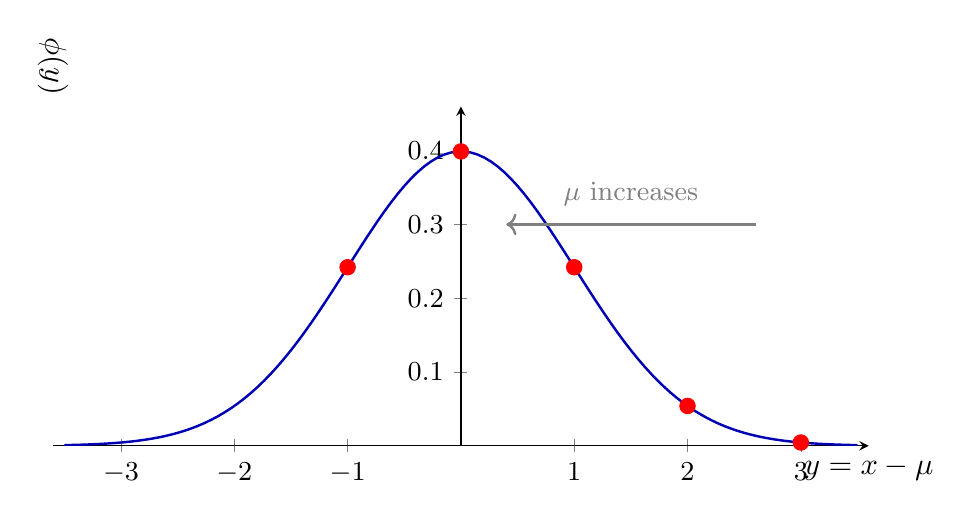
\begin{tikzpicture}[scale=1.1]
  % Draw standard normal curve
  \begin{axis}[
    width=11cm, height=5.5cm,
    domain=-3.5:3.5, samples=120,
    axis lines=center,
    xlabel={$y = x - \mu$},
    ylabel={$\phi(y)$},
    xtick={-3,-2,-1,0,1,2,3},
    ytick={0,0.1,0.2,0.3,0.4},
    ymin=0, ymax=0.46,
    xmin=-3.6, xmax=3.6,
    tick label style={font=\small},
    xlabel style={at={(axis description cs:1,0)},anchor=north},
    ylabel style={at={(axis description cs:0,1)},anchor=east,rotate=-90},
  ]
    \addplot[blue!70!black, thick] {exp(-x^2/2)/sqrt(2*pi)};

    % Dots at y = 3-mu for mu=0,1,2,3,4
    \pgfmathsetmacro{\ya}{3}   % mu=0
    \pgfmathsetmacro{\yb}{2}   % mu=1
    \pgfmathsetmacro{\yc}{1}   % mu=2
    \pgfmathsetmacro{\yd}{0}   % mu=3 (MLE)
    \pgfmathsetmacro{\ye}{-1}  % mu=4

    \addplot[only marks, mark=*, mark size=2.5pt, red]
      coordinates {
        (3,  {exp(-9/2)/sqrt(2*pi)})
        (2,  {exp(-4/2)/sqrt(2*pi)})
        (1,  {exp(-1/2)/sqrt(2*pi)})
        (0,  {1/sqrt(2*pi)})
        (-1, {exp(-1/2)/sqrt(2*pi)})
      };

    % Labels for mu values
    \node[below, font=\tiny, red] at (axis cs:3,-0.01) {$\mu{=}0$};
    \node[below, font=\tiny, red] at (axis cs:2,-0.01) {$\mu{=}1$};
    \node[below, font=\tiny, red] at (axis cs:1,-0.01) {$\mu{=}2$};
    \node[below, font=\tiny, red, fill=yellow!30, rounded corners=2pt]
      at (axis cs:0,-0.01) {$\mu{=}3\;(\hat\mu)$};
    \node[below, font=\tiny, red] at (axis cs:-1,-0.01) {$\mu{=}4$};

    % Arrow showing direction of slide
    \draw[->, gray, thick] (axis cs:2.6,0.3) -- (axis cs:0.4,0.3);
    \node[above, font=\small, gray] at (axis cs:1.5,0.31) {$\mu$ increases};

  \end{axis}
\end{tikzpicture}
\end{center}

\noindent
The \textbf{curve is always the same} $\mathcal{N}(0,1)$ --- the
distribution of the pivot does not depend on $\mu$.
But the \textbf{red dot slides}: at $\mu = 0$ it sits far in the
right tail (low density, low likelihood); at $\mu = 3 = x$ it sits
at the peak (high density, maximum likelihood); at $\mu = 4$ it
has slid to the left tail again (low density).

The likelihood $L_X(\mu) = \phi(x - \mu)$ is literally the height of
the fixed curve at the sliding point.  It depends on $\mu$ through
the position of the dot, not through any change in the curve itself.

\begin{remark}[Verbalization of what ``value depends on parameter'' means]
``The distribution of $Y$ does not depend on $\mu$'' means: the
\emph{shape and position of the curve} are always the same standard
normal, regardless of $\mu$.

``The value of $Y$ depends on $\mu$'' means: fixing the observation
$\omega$ (i.e., fixing $x = X(\omega)$), the number $Y(\omega) =
x - \mu$ \emph{changes} as $\mu$ changes.  We slide along the fixed
curve.

These two facts coexist without contradiction: the curve is fixed
(as a function from $\mathbb{R}$ to $[0,\infty)$), but where on
this curve we read off the likelihood is controlled by $\mu$.
The pivot construction ensures the curve is standard normal;
the parameter $\mu$ controls the reading position.
\end{remark}

\subsubsection*{The BP model: two functions instead of one}

In the location family the Jacobian was~$1$: a shift does not
rescale.  The BP model adds a \emph{scale} that depends on parameters,
which brings in a non-trivial Jacobian.  This is why Boris speaks of
``two functions.''

The pivot is now
\[
  \varepsilon_i
  \;=\;
  \frac{y_i - \beta_0 - \beta_1 x_i}{\sigma_{x_i}},
  \qquad
  \sigma_{x_i}^2 = h(\alpha_0 + \alpha_1 x_i),
\]
and $\varepsilon_i \sim \mathcal{N}(0,1)$ for every $(\beta,\alpha)$
— still a pivot.  The map $(y_i, x_i) \mapsto (\varepsilon_i, x_i)$
has Jacobian $\partial\varepsilon_i/\partial y_i = 1/\sigma_{x_i}$,
now non-trivial.  The likelihood contribution is
\[
  p(y_i|x_i;\beta,\alpha)
  = \phi(\varepsilon_i(\beta,\alpha)) \cdot \frac{1}{\sigma_{x_i}}.
\]
The \textbf{two functions} Boris identifies:
\begin{enumerate}
\item $\phi(\varepsilon_i(\beta,\alpha))$ — the pivot density at the
  observed point; depends on $(\beta,\alpha)$ through the \emph{argument}.
\item $1/\sigma_{x_i}$ — the Jacobian; depends on $\alpha$ through the
  \emph{scale}.
\end{enumerate}
In the location example, function~(2) was identically~$1$ and dropped
out.  Here both contribute to the likelihood, and their product gives
a richer dependence on $(\beta,\alpha)$ than either alone.

The ``compensation'' in the distribution of $\varepsilon_i$ works as
follows: as $(\beta,\alpha)$ change, the numerator $y-\beta_0-\beta_1
x$ and the denominator $\sigma_x$ both change — together they keep
$\varepsilon_i$ standard normal in distribution.  In the likelihood,
fixing $(y_i,x_i)$ breaks this cooperation: the argument and the
Jacobian evolve independently as $(\beta,\alpha)$ vary.



Suppose $\varepsilon_1, \ldots, \varepsilon_n$ are i.i.d.\ $\mathcal{N}(0,1)$.
Their joint density on $\mathbb{R}^n$ is the product of $n$ standard
normal densities:
\[
  p_\varepsilon(\varepsilon_1,\ldots,\varepsilon_n)
  \;=\;
  \prod_{i=1}^n \frac{1}{\sqrt{2\pi}}\,e^{-\varepsilon_i^2/2}
  \;=\;
  (2\pi)^{-n/2}\exp\!\left(-\frac{1}{2}\sum_{i=1}^n \varepsilon_i^2\right).
\]
This is a fixed, parameter-free function on $\mathbb{R}^n$: it does
not depend on $\beta$ or $\alpha$.  Next time we will substitute
$\varepsilon_i = (y_i - \beta_0 - \beta_1 x_i)/\sigma_{x_i}$ into
this expression and account for the Jacobian to obtain the likelihood
$l(\beta,\alpha)$.

\subsubsection*{The concept Boris identifies: likelihood of a pivot}

Boris makes the following observation, which he says he never
encountered explicitly in his studies.

A \textbf{pivot} is a function $T = t(X;\theta)$ of the data $X$ and
the parameter $\theta$ whose distribution does not depend on $\theta$.
The canonical example: if $X \sim \mathcal{N}(\mu,\sigma^2)$, then
$Z = (X-\mu)/\sigma \sim \mathcal{N}(0,1)$ for every $(\mu,\sigma)$
— the distribution of $Z$ is fixed, but $Z$ itself depends on the
unknown parameters.

In our model, $\varepsilon_i = (y_i - \beta_0 - \beta_1 x_i)/\sigma_{x_i}$
is exactly a pivot: for every $(\beta, \alpha)$,
\[
  \varepsilon_i(\beta,\alpha) \;\sim\; \mathcal{N}(0,1).
\]
The distribution does not depend on parameters.  Yet $\varepsilon_i$
itself depends on them through the formula.

Now consider the likelihood.  We evaluate the density of $Y_i$ given
$X_i = x_i$ using the change-of-variables formula:
\[
  p(y_i \mid x_i;\,\beta,\alpha)
  = \underbrace{
      \frac{1}{\sqrt{2\pi}}\,e^{-\varepsilon_i(\beta,\alpha)^2/2}
    }_{\text{pivot density at observed point}}
  \;\cdot\;
  \underbrace{\frac{1}{\sigma_{x_i}}}_{\text{Jacobian}}.
\]
Boris's observation: there are two separate dependencies on the
parameters.
\begin{itemize}
\item The density function $\phi(\,\cdot\,)$ is fixed (does not depend
  on parameters).  But its \emph{argument} $\varepsilon_i(\beta,\alpha)$
  does.
\item The Jacobian $1/\sigma_{x_i}$ depends on $\alpha$ through
  $\sigma_{x_i}^2 = h(\alpha_0 + \alpha_1 x_i)$.
\end{itemize}
Together, these two functions give a non-trivial, parameter-dependent
likelihood — even though the distribution of the pivot is fixed.

\begin{remark}[Why the two dependencies do not cancel in the likelihood]
One might wonder: if the distribution of $\varepsilon_i(\beta,\alpha)$
is always $\mathcal{N}(0,1)$, why does the likelihood depend on $\beta$
and $\alpha$ at all?

The answer is that the distribution being fixed means: if you draw a
new $\varepsilon_i(\beta,\alpha)$ for each $(\beta,\alpha)$, you always
get a $\mathcal{N}(0,1)$ value.  But in the likelihood we do not draw
a new $\varepsilon_i$ — we fix the \emph{observed data} $(y_i, x_i)$
and vary $(\beta,\alpha)$.  Different parameter values assign different
values to $\varepsilon_i(y_i, x_i;\beta,\alpha)$ — some close to zero
(high density), some far (low density).  The likelihood measures how
plausible the observed data are under each parameter value; the pivot
construction is a tool for doing this calculation cleanly.

Concretely: at the true $(\beta_0,\alpha_0)$, the observed $y_i$ was
generated with $\varepsilon_i \approx 0$ (on average), so the density
is high.  At wrong parameter values, the implied $\varepsilon_i$ may
be large, and the density is low.
\end{remark}

\begin{remark}[Boris's formulation: two functions compensating]
Boris writes: ``distribution does not depend on parameters as a
function, but it still appears in its arguments.  Two functions
compensate each other giving the fixed density for the whole family.''

The two functions are: (i) the map $(\beta,\alpha) \mapsto
\varepsilon_i(\beta,\alpha)$ (shifts the argument of $\phi$), and
(ii) the Jacobian $1/\sigma_{x_i}$ (scales the density).  They
compensate in the following precise sense: for any fixed $(\beta,\alpha)$,
the pushforward of the law of $Y_i$ (given $X_i = x_i$) under the
map $y \mapsto (y-\beta_0-\beta_1 x_i)/\sigma_{x_i}$ is $\mathcal{N}(0,1)$.
This is the content of the pivot: the two functions cooperate to
produce a parameter-free distribution.  But in the likelihood, we
evaluate at a fixed $y_i$, not at a draw from the distribution, so
the compensation is broken and the parameter-dependence is exposed.
\end{remark}

\subsubsection*{Plugging in: from joint pivot density to the likelihood}

Boris's homework set up the joint density of $\varepsilon_1,\ldots,
\varepsilon_n$.  The next step: substitute
\[
  \varepsilon_i = \varepsilon_i(\beta,\alpha)
  := \frac{y_i - \beta_0 - \beta_1 x_i}{\sigma_{x_i}},
  \qquad
  \sigma_{x_i}^2 = h(\alpha_0 + \alpha_1 x_i),
\]
and account for the Jacobian of the vector map
$(y_1,\ldots,y_n) \mapsto (\varepsilon_1,\ldots,\varepsilon_n)$:
\[
  \det\!\left(\frac{\partial\varepsilon}{\partial y}\right)
  = \prod_{i=1}^n \frac{1}{\sigma_{x_i}}.
\]
(The map is diagonal, so the Jacobian determinant is the product of
the individual Jacobians.)  The log-likelihood is:
\begin{align*}
  l(\beta,\alpha)
  &= \log p_\varepsilon\!\left(\varepsilon_1(\beta,\alpha),\ldots,
     \varepsilon_n(\beta,\alpha)\right)
   + \log\prod_{i=1}^n\frac{1}{\sigma_{x_i}} \\[4pt]
  &= -\frac{n}{2}\log(2\pi)
   - \frac{1}{2}\sum_{i=1}^n \varepsilon_i(\beta,\alpha)^2
   - \sum_{i=1}^n \log\sigma_{x_i} \\[4pt]
  &= -\frac{n}{2}\log(2\pi)
   - \frac{1}{2}\sum_{i=1}^n \log\sigma_{x_i}^2
   - \frac{1}{2}\sum_{i=1}^n
     \frac{(y_i - \beta_0 - \beta_1 x_i)^2}{\sigma_{x_i}^2},
\end{align*}
which is the BP log-likelihood derived in §\,\ref{subsec:likelihood}
by a different route.  The two routes — direct density of $Y|X$ and
change of variables through the pivot $\varepsilon$ — give identical
results, as they must.

%--------------------------------------------------------------------

\subsection{The general pivot framework and its application to regression}
\label{subsec:pivot-framework}

We follow Boris's notes of July~12, 2026 (note~61).

\subsubsection*{Boris's framework: compensating map}

\paragraph{Setup.}
Let $(\Omega, \mathcal{F})$ be a measurable space.  We have a
random variable
\[
  X \;:\; \Omega \;\longrightarrow\; \mathbb{R},
\]
which is a \emph{fixed} measurable map — it does not depend on
any parameter.  We have a parametrised family of measures on
$\mathbb{R}$:
\[
  \{P_\theta\}_{\theta \in \Theta}.
\]
This family tells us how $X$ is distributed: $X \sim P_\theta$ when
the true parameter is $\theta$.  The variability across $\theta$
lives entirely in the measures $P_\theta$, not in the map~$X$.

Suppose densities exist.  Then $\{P_\theta\}$ is connected to a
parametrised family of densities $\{f_\theta\}$ via a base
(reference) measure on $\mathbb{R}$.  Two standard cases:
\begin{itemize}
\item \textbf{Continuous:} $f_\theta(x)$ is a density with respect
  to Lebesgue measure on $\mathbb{R}$, so $P_\theta(A) =
  \int_A f_\theta(x)\,\mathrm{d}x$.
\item \textbf{Discrete:} $f_\theta(x)$ is a mass function with
  respect to counting measure on some countable set, so
  $P_\theta(A) = \sum_{x \in A} f_\theta(x)$.
\end{itemize}
On $\Omega$ we introduce \emph{no} such base measure and therefore
\emph{no} density on $\Omega$.  We do not have an analogue of
Lebesgue measure sitting on $\Omega$, so the map $X:\Omega\to
\mathbb{R}$ is not a density — it is simply a measurable function.
Densities live on $\mathbb{R}$ (the $x$-axis), not on $\Omega$.

\begin{figure}[ht]
\centering
\includegraphics[width=0.55\textwidth]{fig_61_x.png}
\caption{Boris's diagram (July~12, 2026): the fixed map
$X:\Omega\to\mathbb{R}$ sending $\omega$ to $X(\omega)$.  The oval
is $\Omega$; the green band is the image of $X$.}
\end{figure}

\paragraph{The compensating map.}
We introduce a parametrised family of measurable maps
\[
  g_\theta \;:\; \mathbb{R} \;\longrightarrow\; \mathbb{R}, \qquad
  \theta \in \Theta.
\]
Equivalently, $g$ is a function of two variables: $g: \mathbb{R}
\times \Theta \to \mathbb{R}$.  Define the composed random variable
\[
  Y_\theta(\omega) \;:=\; g_\theta\!\bigl(X(\omega)\bigr).
\]
This is a new random variable, parametrised by $\theta$ through the
map $g_\theta$.

\begin{figure}[ht]
\centering
\includegraphics[width=0.75\textwidth]{fig_61_xy.png}
\caption{Boris's diagram (July~12, 2026): the full composition
$\Omega \xrightarrow{X} \mathbb{R} \xrightarrow{g_\theta}
\mathbb{R}$, sending $\omega \mapsto X(\omega) \mapsto
Y(\omega) = g_\theta(X(\omega))$.  The second axis (red) carries
$Y(\omega)$.}
\end{figure}

Its distribution is the pushforward
\[
  Q_\theta \;:=\; (g_\theta)_* P_\theta,
\]
meaning $Q_\theta(B) = P_\theta(\{x : g_\theta(x) \in B\})$ for any
Borel set~$B$.

\paragraph{Definition of a pivot.}
If $Q_\theta$ does not depend on $\theta$ — that is, the image of
the whole measure family $\{P_\theta\}$ under $\{g_\theta\}$ is a
single measure $Q$ — then $Y_\theta$ is called a
\textbf{pivot variable} (or \textbf{pivotal quantity}) with respect
to the family $\{P_\theta\}$:
\[
  (g_\theta)_* P_\theta \;=\; Q \quad \text{for all } \theta \in \Theta.
\]
The family $\{g_\theta\}$ is the \emph{compensating map}: it
corrects for the variation in $P_\theta$ so that the resulting
distribution is always~$Q$.

\paragraph{Why pivot values must depend on $\theta$.}
Boris raises the point from note~60: while the \emph{distribution}
of $Y_\theta$ is parameter-free, its \emph{value}
$Y_\theta(\omega) = g_\theta(X(\omega))$ generically depends on
$\theta$.  The abstract framework makes this a necessity, not an
accident.

Suppose $g_\theta$ is non-trivial: there exist $\theta \neq
\theta'$ and a set $A$ with $P_\theta(A) > 0$ such that
$g_\theta \neq g_{\theta'}$ on $A$.  Since
$(g_\theta)_* P_\theta = (g_{\theta'})_* P_{\theta'} = Q$
but $P_\theta \neq P_{\theta'}$ (the family is non-trivial), the
map $g_\theta$ must absorb the difference between $P_\theta$ and
$P_{\theta'}$.  That absorption is precisely the variation in
$g_\theta$.  For a fixed $\omega$, the value $g_\theta(X(\omega))$
must therefore vary with $\theta$ — otherwise the compensation is
impossible.

\begin{remark}[Boris's range example]
Boris proposes abstracting from the measure to a simpler operator,
for instance the range $\mathrm{rng}(P) = \max - \min$ of the
support.  If $P_\theta$ has range $r(\theta)$, one could choose
$g_\theta(x) = x/r(\theta)$ to stabilise the range of $Q_\theta$.
The map still depends on $\theta$ — the compensating dependence is
unavoidable.  Similarly, for symmetric distributions $p \sim
\mathcal{N}(0,\sigma^2)$, the map $x \mapsto -x$ preserves the
distribution but changes values.
\end{remark}

%--------------------------------------------------------------------

\subsubsection*{The Probabilist's framework: inverse map}

The Probabilist proposes a dual viewpoint that starts from the other end.

\paragraph{Setup.}
Fix a single measure $P$ on $\Omega$ and a single fixed map
\[
  X \;:\; \Omega \;\longrightarrow\; \mathbb{R}.
\]
The distribution of $X$ is fixed: $P_X := X_* P$ is a single
measure on $\mathbb{R}$ that does not depend on any parameter.
Think of $X$ as the ``primordial'' randomness — a standard source
of noise.

\paragraph{The generating map.}
Now introduce the same family $\{g_\theta : \mathbb{R} \to
\mathbb{R}\}_{\theta \in \Theta}$.  Define the composed variable
\[
  Y_\theta(\omega) \;:=\; g_\theta\!\bigl(X(\omega)\bigr).
\]
In the Probabilist's framework, the distribution of $Y_\theta$ \emph{does}
depend on $\theta$, because $g_\theta$ introduces the parameter:
\[
  Q_\theta := (g_\theta)_* P_X \quad \text{varies with } \theta.
\]
The family $\{Q_\theta\}$ is the observed distribution family.
We observe $Y$ (the data), and $X$ is latent.

\paragraph{Recovery: the pivot.}
If $g_\theta$ is invertible (for each $\theta$), we can recover $X$
from $Y_\theta$ by the inverse map:
\[
  X(\omega) \;=\; g_\theta^{-1}\!\bigl(Y_\theta(\omega)\bigr).
\]
Substituting the observed $Y = y$:
\[
  x \;=\; g_\theta^{-1}(y).
\]
The quantity $g_\theta^{-1}(Y)$ — which depends on both the
observation $Y$ and the parameter $\theta$ — has a fixed
distribution $P_X$ regardless of $\theta$.  So $g_\theta^{-1}(Y)$
is the pivot: it is $X$ itself, reconstructed from the data.

\begin{remark}[Comparing the two frameworks]
The two frameworks are dual and connected by the invertibility of
$g_\theta$:
\begin{center}
\small
\begin{tabular}{lll}
\toprule
 & Boris's framework & the Probabilist's framework \\
\midrule
Primary object & $\{P_\theta\}$ on $\mathbb{R}$ & Fixed $P$ on $\Omega$ \\
Fixed quantity & Map $X$ & Map $X$, measure $P$ \\
$g_\theta$ role & Compensating (reduces to $Q$) & Generating (produces $\{Q_\theta\}$) \\
Pivot & $Y_\theta = g_\theta(X)$, dist.\ $Q$ & $X = g_\theta^{-1}(Y)$, dist.\ $P_X$ \\
What we observe & $X \sim P_\theta$ & $Y \sim Q_\theta$ \\
\bottomrule
\end{tabular}
\end{center}
In Boris's framework the pivot lives on the \emph{output} of $g_\theta$;
in the Probabilist's framework the pivot lives on the \emph{input} of $g_\theta$,
recovered by inversion.  They are two descriptions of the same
mathematical object.
\end{remark}

%--------------------------------------------------------------------

\subsubsection*{Application to basic regression}

We apply both frameworks to the simplest regression model:
one-dimensional, no heteroscedasticity.

\paragraph{The model.}
Observe $(X_1, Y_1), \ldots, (X_n, Y_n)$ where
\[
  Y_i \;=\; \beta_0 + \beta_1 X_i + \sigma\,\varepsilon_i,
\]
with $X_i$ fixed design points and $\varepsilon_i \stackrel{\mathrm{iid}}{\sim}
\mathcal{N}(0,1)$.  The parameter is $\theta = (\beta_0, \beta_1, \sigma)$.

\paragraph{The Probabilist's framework fits naturally.}
Set $\Omega = \mathbb{R}^n$, the fixed measure $P =
\mathcal{N}(0,1)^{\otimes n}$, and the fixed random vector
\[
  \varepsilon = (\varepsilon_1, \ldots, \varepsilon_n)
  \;:\; \Omega \;\longrightarrow\; \mathbb{R}^n.
\]
The distribution of $\varepsilon$ under $P$ is $\mathcal{N}(0,
I_n)$ — fixed, no parameters.  This is the ``primordial'' source
of randomness.

The generating map $g_\theta : \mathbb{R}^n \to \mathbb{R}^n$ is
\[
  g_\theta(\varepsilon_1, \ldots, \varepsilon_n)
  \;=\;
  (\beta_0 + \beta_1 X_1 + \sigma\varepsilon_1,\;\ldots,\;
   \beta_0 + \beta_1 X_n + \sigma\varepsilon_n)
  \;=: Y.
\]
The observation $Y = g_\theta(\varepsilon)$ has distribution
$\mathcal{N}(\beta_0 \mathbf{1} + \beta_1 \mathbf{x},\, \sigma^2 I_n)$
— depending on $\theta$.  The pivot is recovered by inversion:
\[
  \varepsilon_i
  \;=\;
  g_\theta^{-1}(Y)_i
  \;=\;
  \frac{Y_i - \beta_0 - \beta_1 X_i}{\sigma}.
\]
This quantity has distribution $\mathcal{N}(0,1)$ for every $\theta$
— it is the pivot.  In regression language: \emph{the standardised
errors are the pivot.}

\paragraph{Boris's framework for the same model.}
The observed quantity is $Y$ with distribution family
$\{P_\theta\}_{\theta \in \Theta}$ where
$P_\theta = \mathcal{N}(\beta_0 \mathbf{1} + \beta_1\mathbf{x},\,
\sigma^2 I_n)$.

The compensating map:
\[
  g_\theta(y_1, \ldots, y_n)
  \;=\;
  \left(\frac{y_1 - \beta_0 - \beta_1 X_1}{\sigma},\;\ldots,\;
  \frac{y_n - \beta_0 - \beta_1 X_n}{\sigma}\right).
\]
The pushforward $(g_\theta)_* P_\theta = \mathcal{N}(0, I_n)$ for
all $\theta$ — a single fixed measure.  So $g_\theta(Y)$ is the
pivot.

Both frameworks give the same pivot $\varepsilon_i = (Y_i -
\beta_0 - \beta_1 X_i)/\sigma$, differing only in which direction
the map $g_\theta$ is applied.  The Probabilist's framework starts from
$\varepsilon$ and generates $Y$; Boris's framework starts from $Y$
and maps back to $\varepsilon$.

\paragraph{Why the pivot values depend on $\theta$.}
For a fixed draw $\omega$ (i.e., a fixed $\varepsilon_i = c$),
the observation is $Y_i(\omega) = \beta_0 + \beta_1 X_i + \sigma c$,
which depends on $\theta$.  Conversely, for a fixed observation
$Y_i = y$, the pivot value is $\varepsilon_i = (y - \beta_0 -
\beta_1 X_i)/\sigma$, which also depends on $\theta$.

The compensating structure: when $\sigma$ increases, $P_\theta$
spreads out (larger variance), but $g_\theta$ divides by the larger
$\sigma$, squeezing the distribution back to $\mathcal{N}(0,1)$.
When $\beta_0$ shifts, $P_\theta$ shifts, but $g_\theta$ subtracts
the shift.  Each change in $\theta$ deforms $P_\theta$, and $g_\theta$
counteracts this deformation.  The values $g_\theta(y)$ must change
with $\theta$ for this counteraction to work — exactly Boris's point
from note~61.

\begin{remark}[The BP pivot as the next step]
In basic regression, both the location ($\beta$) and scale ($\sigma$)
are constant across observations: the same $(\beta_0,\beta_1,\sigma)$
applies to every $i$.  The compensating map $g_\theta$ is the same
function applied to each $(Y_i, X_i)$ pair.

In the BP model, the scale $\sigma_i = \sqrt{h(\alpha_0 + \alpha_1
X_i)}$ varies with $X_i$.  The compensating map becomes
\[
  g_\theta(Y_i, X_i)
  \;=\;
  \frac{Y_i - \beta_0 - \beta_1 X_i}{\sqrt{h(\alpha_0 + \alpha_1 X_i)}},
\]
where now $g_\theta$ depends on \emph{two} parameter blocks: $\beta$
(through the location) and $\alpha$ (through the scale function $h$).
The pivot $\varepsilon_i = g_\theta(Y_i, X_i)$ is still
$\mathcal{N}(0,1)$ for all $(\beta,\alpha)$ — but recovering it from
the data requires knowing (or estimating) both parameter blocks.
\end{remark}

%--------------------------------------------------------------------

\subsection{Pivot in regression: the score argument}
\label{subsec:pivot-score}

We follow Boris's notes of July~13, 2026 (note~62).

\subsubsection*{Basic regression: did I construct a pivot?}

Boris considers the single-observation model:
\[
  Y = \beta_0 + \beta_1 X + U, \qquad U = \sigma\varepsilon,
  \qquad \varepsilon \sim \mathcal{N}(0,1),
\]
where $\sigma > 0$ is a deterministic constant (not random).
Expressing $\varepsilon$ through the observables:
\[
  \varepsilon = \frac{Y - \beta_0 - \beta_1 X}{\sigma}.
\]
Boris asks: did I construct a pivot?

\textbf{The Probabilist:} Yes --- but it is a tautology.  The model
\emph{defines} $\varepsilon = U/\sigma$, so the standardised error
is parameter-free by construction.  There is nothing to prove: the
pivot property follows immediately from the definition.

Nevertheless, the construction is correct.  For $n$ observations
indexed by $i$, the pivot values are
\[
  \varepsilon_i = \frac{Y_i - \beta_0 - \beta_1 X_i}{\sigma},
  \qquad i = 1,\ldots,n,
\]
each $\mathcal{N}(0,1)$ independently of the parameter
$(\beta_0, \beta_1, \sigma)$.

\subsubsection*{The BP pivot}

Boris's hypothesis: the BP pivot for observation $i$ is
\[
  \varepsilon_i = \frac{Y_i - \beta_0 - \beta_1 X_i}
                        {\sqrt{h(\alpha^\top z_i)}}.
\]
\textbf{The Probabilist:} Yes, this is correct --- provided $h(\cdot)$ is
parametrised by $\alpha$.  Each $\varepsilon_i$ is
$\mathcal{N}(0,1)$ for every $(\beta,\alpha)$.

However, the Probabilist notes a conceptual jump: in basic regression,
$\sigma$ is a constant (deterministic, the same for all $i$).
In the BP model, $\sigma_i = \sqrt{h(\alpha^\top z_i)}$ varies
with $i$ because $z_i$ varies --- and if $z_i = x_i$ is a
realisation of a random $X_i$, then $\sigma_i$ is itself random.
This is the transition from deterministic to random scale discussed
in notes~50--51.

\subsubsection*{Why the score is not flat zero: the key argument}

Boris: if $\varepsilon \sim \mathcal{N}(0,1)$ and its density does
not depend on parameters, then its score is identically zero.  So
where does the non-trivial score come from?

\textbf{The Probabilist:} If we \emph{observed} $\varepsilon_i$ directly, then
yes --- the likelihood would be
\[
  L(\varepsilon_1,\ldots,\varepsilon_n)
  = \prod_{i=1}^n \phi(\varepsilon_i),
\]
which contains no parameters.  The score with respect to any
$\theta$ would be identically zero.  But we do not observe
$\varepsilon_i$.  We observe $Y_i$ and $X_i$.

The resolution: $\varepsilon_i$ is not a free variable --- it is a
\emph{function} of the observed data and the unknown parameters:
$\varepsilon_i = \varepsilon_i(Y_i, X_i;\,\theta)$.  When we
substitute this expression into the likelihood, the parameters
reappear through the argument of $\phi$.

\subsubsection*{Abstract formulation: composition of two functions}

The Probabilist states the argument abstractly.  Let $f$ be a function (the
density $\phi$) and let $g_\theta$ be the pivot map (depending on
$\theta$).  Consider the composition
\[
  h(\theta) \;:=\; f\!\bigl(g_\theta(y)\bigr).
\]
This composition depends on $\theta$ --- so its derivative with
respect to $\theta$ is generally non-zero.

Set $\eta := g_\theta(y)$ (the pivot value at the observation $y$).
There are two ways to look at $\eta$:

\textbf{View~1 --- $\eta$ as an independent variable.}  Treat
$\eta$ as a free number.  Then
\[
  \frac{\partial f}{\partial \eta}(\eta) = \phi'(\eta) = -\eta\,\phi(\eta).
\]
This is a property of $f$ alone; no $\theta$ involved.

\textbf{View~2 --- $\eta$ as a dependent variable} ($\eta =
g_\theta(y)$, function of $\theta$).  By the chain rule:
\[
  \frac{\partial}{\partial\theta}\,f(g_\theta(y))
  = f'(g_\theta(y))\cdot \frac{\partial g_\theta(y)}{\partial\theta}
  = \phi'(\varepsilon(\theta))\cdot\frac{\partial\varepsilon}{\partial\theta}.
\]
This is generally non-zero because $\partial\varepsilon/\partial\theta
\neq 0$: the pivot value changes when $\theta$ changes (it must, to
keep the distribution fixed).

In regression, $\varepsilon_i(\theta) = (y_i - \beta_0 -
\beta_1 x_i)/\sigma$ gives
\[
  \frac{\partial\varepsilon_i}{\partial\beta_0} = -\frac{1}{\sigma},
  \qquad
  \frac{\partial\varepsilon_i}{\partial\beta_1} = -\frac{x_i}{\sigma},
  \qquad
  \frac{\partial\varepsilon_i}{\partial\sigma}
  = -\frac{y_i - \beta_0 - \beta_1 x_i}{\sigma^2}
  = -\frac{\varepsilon_i}{\sigma}.
\]
None of these are zero in general.

\subsubsection*{The log-likelihood through substitution}

Substituting $\varepsilon_i = (y_i - \beta_0 - \beta_1 x_i)/\sigma$
into the joint density of $(\varepsilon_1,\ldots,\varepsilon_n)$
and including the Jacobian $\prod_i (1/\sigma)$, the likelihood is:
\[
  L(\beta_0,\beta_1,\sigma;\,y_1,\ldots,y_n)
  = \prod_{i=1}^n \phi\!\left(\frac{y_i-\beta_0-\beta_1 x_i}{\sigma}\right)
    \cdot\frac{1}{\sigma}.
\]
Taking logarithms, the log-likelihood is
\begin{align*}
  l(\beta_0,\beta_1,\sigma)
  &= \sum_{i=1}^n \log\phi(\varepsilon_i) - n\log\sigma \\[4pt]
  &= -\frac{n}{2}\log(2\pi)
     - \frac{1}{2}\sum_{i=1}^n \varepsilon_i^2
     - n\log\sigma \\[4pt]
  &= -\frac{n}{2}\log(2\pi)
     - n\log\sigma
     - \frac{1}{2\sigma^2}\sum_{i=1}^n(y_i - \beta_0 - \beta_1 x_i)^2.
\end{align*}
This is the standard normal regression log-likelihood, and it
manifestly depends on $(\beta_0, \beta_1, \sigma)$ through both
the residuals and the $-n\log\sigma$ term.

\begin{remark}[The two contributions to the score]
Differentiating $l$ with respect to $\beta_0$:
\[
  \frac{\partial l}{\partial\beta_0}
  = \frac{1}{\sigma^2}\sum_{i=1}^n (y_i - \beta_0 - \beta_1 x_i)
  = \frac{1}{\sigma}\sum_{i=1}^n\varepsilon_i.
\]
This is the chain rule in action: $\partial l/\partial\beta_0 =
\sum_i (\partial\log\phi/\partial\varepsilon_i)\cdot
(\partial\varepsilon_i/\partial\beta_0) = \sum_i (-\varepsilon_i)
\cdot(-1/\sigma)$.

The score is zero at the MLE $\hat\beta_0$ because $\sum_i
\hat\varepsilon_i = 0$ (OLS residuals sum to zero).  This is
exactly the condition that the true $\varepsilon_i$ are centered
--- it holds at the MLE, not in general.
\end{remark}

%--------------------------------------------------------------------

\subsection{Transformed likelihood and non-injectivity of the pivot map}
\label{subsec:transformed-likelihood}

We follow Boris's notes of July~14, 2026 (note~63).

\subsubsection*{Likelihood as probability of the observed event}

For a cleaner conceptual foundation, start in the discrete case.
Let $X_1,\ldots,X_n$ be i.i.d.\ with probability mass function
$p(x;\theta) = P_\theta\{X = x\}$.  The likelihood is
\[
  L(\theta;\,x_1,\ldots,x_n)
  = p(x_1;\theta)\cdots p(x_n;\theta)
  = P_\theta\{X_1 = x_1,\,\ldots,\,X_n = x_n\}.
  \tag{1}
\]
This has a direct interpretation: it is the probability, under
measure $P_\theta$, of observing the exact values we did.
The MLE is the $\theta$ that makes this probability largest ---
it selects the measure under which the observed data are most
plausible.

\subsubsection*{Transformed likelihood: the bijective case}

Suppose there is a transformation $g$ such that $g(X)$ has a more
standard or tractable distribution (e.g.\ a pivot).  Consider the
alternative expression
\[
  P_\theta\{g(X_1) = g(x_1),\,\ldots,\,g(X_n) = g(x_n)\}.
  \tag{2}
\]
\textbf{If $g$ is bijective:} the events in (1) and (2) are
identical --- $g(X_i) = g(x_i) \Leftrightarrow X_i = x_i$ ---
so (1) and (2) are the same number, and maximising either over
$\theta$ gives the same MLE.  The benefit is purely
presentational: the distribution of $g(X)$ may be tabulated or
familiar, making it easier to work with.

\subsubsection*{Regression: the map is not injective}

In the regression setting, the observed unit is the pair
$(X_i, Y_i) \in \mathbb{R}^2$.  Its joint distribution depends on
$(\beta_0, \beta_1)$ and on the unknown marginal distribution of
$X_i$ --- which we do not specify.  Writing the joint likelihood of
$(x_i, y_i)$ pairs directly is therefore impossible.

The natural transformation is
\[
  g_\beta(x, y) \;=\; y - \beta_0 - \beta_1 x \;=\; \varepsilon,
\]
a map $g_\beta : \mathbb{R}^2 \to \mathbb{R}$.  Under this map,
the residual $\varepsilon_i = Y_i - \beta_0 - \beta_1 X_i$ has
distribution $\mathcal{N}(0,\sigma^2)$ --- one parameter instead
of the original three $(\beta_0,\beta_1,\sigma)$.  The parameters
$\beta_0$ and $\beta_1$ have been ``absorbed'' into the
transformation; only $\sigma$ remains visible.

Moreover, $\varepsilon_1,\ldots,\varepsilon_n$ are i.i.d.\ (because
$(X_i,Y_i)$ are i.i.d.\ and the transformation is the same for
each $i$), so the transformed likelihood is again a product:
\[
  L(\sigma;\,\varepsilon_1(\beta),\ldots,\varepsilon_n(\beta))
  = \prod_{i=1}^n f_\sigma(\varepsilon_i(\beta)).
\]

\subsubsection*{The problem: $g_\beta$ is not injective}

Here a conceptual difficulty arises.  The map
$g_\beta : \mathbb{R}^2 \to \mathbb{R}$ is affine and
\emph{reduces dimension}, so it cannot be injective:

\begin{itemize}
\item If $\beta_1 = 0$: any two pairs $(y, x_1)$ and $(y, x_2)$
  with the same $y$ map to the same value $y - \beta_0$.
  Non-injectivity is obvious.
\item If $\beta_1 \neq 0$: the kernel of the linear part of $g_\beta$
  is the line $\{(x,y) : y = \beta_1 x\}$ in $\mathbb{R}^2$.
  Every fibre $g_\beta^{-1}(\varepsilon)$ is the line
  $\{(x,y) : y - \beta_0 - \beta_1 x = \varepsilon\}$ --- an
  infinite set.  Injectivity fails.
\end{itemize}

Since any linear map from $\mathbb{R}^2$ to $\mathbb{R}$ has a
non-trivial kernel, injectivity is structurally impossible.

\textbf{Consequence for the likelihood.}
The equivalence between (1) and (2) required bijectivity.  Without
it, the event $\{g_\beta(X_i,Y_i) = \varepsilon_i\}$ contains
infinitely many pairs, while the event
$\{(X_i,Y_i) = (x_i,y_i)\}$ is a single point.  So
\[
  P_\theta\{g_\beta(X_i,Y_i) = \varepsilon_i\}
  \;\neq\;
  P_\theta\{(X_i,Y_i) = (x_i,y_i)\},
\]
and the MLE from the transformed likelihood is generally
\emph{different} from the MLE of the original.

\subsubsection*{Resolution: it is the only likelihood we can write}

Boris identifies the resolution.  Although the transformed
likelihood is not equivalent to the joint likelihood of $(X_i,Y_i)$
pairs, it is \emph{the only likelihood available in this model}.
The reason: we place no restrictions on the marginal distribution
of~$X_i$.  The distribution of $X$ is a completely free
infinite-dimensional nuisance.  Without specifying it, the joint
distribution of $(X_i,Y_i)$ cannot be written down, and neither can
the full joint likelihood~(1).

What \emph{can} be written is the conditional likelihood:
\[
  L_{\mathrm{cond}}(\beta,\sigma;\,y_1,\ldots,y_n \mid x_1,\ldots,x_n)
  = \prod_{i=1}^n f_{Y|X}(y_i \mid x_i;\,\beta,\sigma)
  = \prod_{i=1}^n \frac{1}{\sigma}\,
    \phi\!\left(\frac{y_i - \beta_0 - \beta_1 x_i}{\sigma}\right).
\]
This is exactly the product of the transformed densities (with
Jacobian $1/\sigma$ from dividing by~$\sigma$).  Maximising this
over $(\beta,\sigma)$ gives OLS estimates of $\beta$ and an
estimate of $\sigma^2$ --- the standard regression procedure.

\begin{remark}[Why the non-injectivity does not invalidate the method]
The non-injectivity of $g_\beta$ means the transformed likelihood
is not the same number as the joint likelihood.  But we are not
claiming equivalence to a joint likelihood that we cannot write
anyway.  We are simply maximising the conditional likelihood, which
is the natural object given that the marginal distribution of $X$
is unspecified.  The OLS estimator $\hat\beta$ is the MLE of this
conditional likelihood, and it has the usual optimal properties
under the model assumptions.
\end{remark}

\begin{remark}[Connection to the pivot framework]
In the language of §\,\ref{subsec:pivot-framework}, the map
$g_\beta(x,y) = y - \beta_0 - \beta_1 x$ is Boris's compensating
map restricted to the $y$-direction.  It sends the family of
conditional distributions $\{f_{Y|X=x}(\cdot\,;\beta)\}$ to the
fixed distribution $\mathcal{N}(0,\sigma^2)$.  The Jacobian of
the inverse (from $\varepsilon$ back to $y$, holding $x$ fixed)
is $\sigma$ --- this is where the $1/\sigma$ factor in the
conditional density comes from.
\end{remark}

%--------------------------------------------------------------------

\subsection{Likelihood as a surface and random curtains}
\label{subsec:random-curves}

We follow Boris's notes of July~15, 2026 (note~64).

\subsubsection*{The likelihood surface}

For the location-normal family with a single observation, both the
parameter $\mu$ and the observation $x$ are real numbers.  The
likelihood can be viewed as a function of \emph{both} simultaneously:
\[
  L(x,\mu) \;=\; \phi(x - \mu)
  \;=\; \frac{1}{\sqrt{2\pi}}\,e^{-(x-\mu)^2/2}.
\]
Boris notes this is not the standard view --- usually one fixes the
observation and varies $\mu$, or fixes $\mu$ and varies $x$ ---
but looking at the full surface is valid and illuminating.

The surface $L(x,\mu)$ lives over the $(x,\mu)$-plane.  It has the
shape of a ridge: a bell-shaped hill running along the diagonal
$x = \mu$, falling off on both sides.  Two natural cross-sections:

\begin{itemize}
\item \textbf{Fix $\mu = \mu_0$, vary $x$:} the section
  $x \mapsto \phi(x-\mu_0)$ is the density of $\mathcal{N}(\mu_0,1)$
  --- a bell centred at $x = \mu_0$.

\item \textbf{Fix $x = x_0$, vary $\mu$:} the section
  $\mu \mapsto \phi(x_0-\mu)$ is the likelihood at observation $x_0$
  --- a bell centred at $\mu = x_0$.
\end{itemize}

Boris observes: both sections have the \emph{same shape}.  The Probabilist's
explanation: for any symmetric location family with density
$f_0(x-\mu)$, the two sections are
\[
  f_0(x - \mu_0) \quad\text{(density section)}
  \qquad\text{and}\qquad
  f_0(x_0 - \mu) = f_0(-({\mu - x_0})) = f_0(\mu - x_0)
  \quad\text{(likelihood section).}
\]
When $f_0$ is symmetric ($f_0(-z) = f_0(z)$), both equal $f_0$ of
the absolute difference $|x - \mu|$, giving identical shapes.
This holds for the normal and the Cauchy, but not for asymmetric
families (exponential, Poisson): for those, the density and
likelihood cross-sections have different shapes.

\begin{figure}[H]
\centering
\includegraphics[width=0.72\textwidth]{fig64_1_surface.png}
\caption{Boris's diagram~1 (July~15, 2026): the 3D surface
$L(x,\mu) = \phi(x-\mu)$ over the $(x,\mu)$-plane.  The ridge
runs along the diagonal $x = \mu$.  Sections by fixed $x$ give
densities; sections by fixed $\mu$ give likelihoods --- both are
bell-shaped with the same width.}
\end{figure}

\subsubsection*{Orange curtains: random likelihood curves}

Fix the true parameter $\mu_t$.  Sample observations
$x_1, x_2, \ldots$ from $\mathcal{N}(\mu_t, 1)$.  Each observation
$x_i$ is a point on the $x$-axis; Boris draws them as orange dots,
dense near $\mu_t$ and sparse far from it (reflecting the bell-shaped
sampling density).

Each observation $x_i$ generates a likelihood curve:
$\mu \mapsto \phi(x_i - \mu)$ --- a bell centred at $\mu = x_i$.
Boris calls these the \textbf{orange curtains}: vertical slices of
the surface $L(x,\mu)$ at $x = x_i$, ``hanging'' from the ridge.
Since observations $x_i$ cluster near $\mu_t$, the orange curtains
also cluster near $\mu_t$, and their peaks concentrate around
$\mu = \mu_t$.

\begin{figure}[H]
\centering
\includegraphics[width=0.72\textwidth]{fig64_2_points.png}
\caption{Boris's diagram~2: the same surface $\phi(x-\mu)$ with
orange sample points drawn from $\mathcal{N}(\mu_t,1)$ on the
$x$-axis.  Each point gives rise to an orange likelihood curtain.
Curtains cluster near $\mu_t$.}
\end{figure}

\begin{remark}[Naming ``true'' vs.\ ``abstract'' $\mu$]
Boris notes the need to distinguish two roles of $\mu$.  The
\emph{true} parameter $\mu_t$ is fixed and governs the sampling of
$x$.  The \emph{abstract} (or hypothetical, or dummy) $\mu$ is the
variable over which we draw the likelihood curve.  In frequentist
statistics there is no standard single name for the dummy $\mu$;
it is often called the ``parameter argument'' or simply ``the
parameter'' with the understanding that the likelihood is a function
of it.  The true $\mu_t$ is a fixed unknown constant, not a variable.
\end{remark}

\subsubsection*{The pivot surface}

Now apply the pivot map $g_\mu(x) = x - \mu$.  Boris stresses: here
$\mu$ is the abstract parameter, not necessarily the true one.
Viewed as a function of two variables $(x, \mu)$, the map
\[
  g : (x, \mu) \;\mapsto\; y = x - \mu
\]
is a \emph{plane} --- it is linear (affine) in both $x$ and $\mu$
simultaneously.  This plane tilts at $45°$ across the
$(x,\mu)$-plane: where $x > \mu$ the output is positive; where
$x < \mu$ it is negative; the zero-set is the diagonal $x = \mu$.

\begin{figure}[H]
\centering
\includegraphics[width=0.52\textwidth]{fig64_3_2d.png}
\caption{Boris's diagram~3: the 2D map $y = x - \mu$ as a function
of $(x,\mu)$.  The shading shows positive (blue) and negative (red)
regions separated by the diagonal $x = \mu$ where $y = 0$.}
\end{figure}

\begin{figure}[H]
\centering
\includegraphics[width=0.72\textwidth]{fig64_4_gplane.png}
\caption{Boris's diagram~4: $g_\mu(x) = x - \mu$ as a 3D surface
over the $(x,\mu)$-plane.  It is a tilted plane (not a curved
surface), rising along $x$ and falling along $\mu$.}
\end{figure}

The substitution $y = x - \mu$ changes variables in the likelihood
surface:
\[
  L(x,\mu) = \phi(x-\mu) = \phi(y).
\]
In the new coordinate $y$, the likelihood is simply $\phi(y)$ ---
a function of $y$ alone, with \emph{no $\mu$ anywhere}.

\subsubsection*{Green curtains: horizontal after the transform}

Take any fixed true value, say $\mu_t = 5$, and sample
$x \in \{4,\, 4.5,\, 5.1\}$.  Under the pivot map at $\mu = \mu_t$:
\[
  y_i = x_i - 5 \;\in\; \{-1,\,-0.5,\,0.1\}.
\]
Each transformed value $y_i$ gives a ``green curtain'' on the
$(y,\mu)$-surface: the function $\mu \mapsto \phi(y_i)$.  But
$\phi(y_i)$ does not depend on $\mu$ --- it is a constant as $\mu$
varies.  The curtain is a \textbf{horizontal plane}: the same height
everywhere along the $\mu$-axis.

\begin{figure}[H]
\centering
\includegraphics[width=0.72\textwidth]{fig64_5_phiy.png}
\caption{Boris's diagram~5: the surface $\phi(y)$ over the
$(y,\mu)$-plane.  The green curtains at fixed values of $y$ are
horizontal --- $\phi(y)$ does not depend on $\mu$.  Compare with
diagram~2: the orange curtains were bell-shaped; the green curtains
are flat.}
\end{figure}

\begin{remark}[The visual statement of the pivot property]
In the original $(x,\mu)$ space, the orange curtain at observation
$x_i$ is a bell curve in $\mu$ --- it rises, peaks at $\mu = x_i$,
and falls.  Picking a different $\mu$ gives different likelihood
values.

After the pivot transform, the green curtain at $y_i = x_i - \mu_t$
is a horizontal line --- the same value $\phi(y_i)$ regardless of
$\mu$.  This is the geometric meaning of ``the distribution of the
pivot does not depend on the parameter'': the likelihood (as a
function of the abstract $\mu$) is flat.

Boris captures the key paradox: \emph{the result does not depend
on $\mu$, but the transform did depend on $\mu$}.  Specifically,
the $y_i = x_i - \mu_t$ were computed using the true $\mu_t = 5$.
If we had used a different $\mu_t$, we would have gotten different
$y_i$'s --- the \emph{values} would be different.  Yet for any
fixed $y_i$, the function $\mu \mapsto \phi(y_i)$ is flat.  The
transform carries the $\mu$-dependence into the \emph{value} of
$y_i$; the standard normal density $\phi$ then displays that value
without any further $\mu$-dependence.

This is the same observation from note~60, now seen geometrically:
fixing $\omega$ (the randomness) fixes $x$, which fixes $y = x -
\mu_t$ at a particular value; the flat curtain at that value is the
horizontal section of $\phi$.  The distribution of $y$ over random
$\omega$ is $\mathcal{N}(0,1)$ regardless of $\mu_t$ --- but which
value $y$ takes does depend on $\mu_t$.
\end{remark}

%--------------------------------------------------------------------

\FloatBarrier
%--------------------------------------------------------------------

\subsection{Regular conditional distribution and the conditional likelihood of \texorpdfstring{$Y \mid X$}{Y|X}}
\label{subsec:rcd-likelihood}

We follow Boris's notes of July~17, 2026 (note~65).

\subsubsection*{The conditioning problem}

The model specifies the conditional distribution of $U$ given $X$:
\[
  U \mid X = x \;\sim\; \mathcal{N}(0,\,\sigma^2(x)),
  \qquad \sigma^2(x) = h(\alpha_0 + \alpha_1 x).
\]
For continuous $X$, the event $\{X = x\}$ has probability zero.
The conditional probability $P(U \in A \mid X = x)$ cannot be
defined as a ratio $P(U \in A,\, X = x)/P(X = x)$ — the denominator
is zero.  For each individual $x$ one can find a version of the
conditional probability defined up to a $P_X$-null set.  The
difficulty: \emph{there is no single null set that works for
all~$x$ simultaneously} in general.

\subsubsection*{Regular conditional distribution}

For abstract probability spaces this is a genuine obstruction, and
counterexamples exist.  However, for Polish spaces such as
$\mathbb{R}$ or $\mathbb{R}^d$, a canonical simultaneous version
always exists.

\begin{definition}
A \textbf{regular conditional distribution} of $U$ given $X$ is a
function
\[
  \kappa : \Omega \times \mathcal{B}(\mathbb{R}) \;\longrightarrow\; [0,1]
\]
satisfying:
\begin{enumerate}
\item For every fixed $\omega \in \Omega$: the map $A \mapsto
  \kappa(\omega, A)$ is a probability measure on $\mathbb{R}$.
\item For every fixed Borel set $A \in \mathcal{B}(\mathbb{R})$:
  the map $\omega \mapsto \kappa(\omega, A)$ is
  $\sigma(X)$-measurable.
\item $\kappa(\omega, A) = P(U \in A \mid X)(\omega)$ \quad
  $P$-almost surely.
\end{enumerate}
\end{definition}

The map $\omega \mapsto \kappa(\omega, \cdot)$ is a \emph{random
measure} — it assigns a probability measure on $\mathbb{R}$ to
each sample point~$\omega$.  Condition~(1) ensures it is a proper
measure for each $\omega$; condition~(2) ensures it is measurable.

In our model, writing $x = X(\omega)$, the regular conditional
distribution takes the specific form
\[
  \kappa(\omega, A)
  = \mathcal{N}\!\bigl(0,\; h(\alpha_0 + \alpha_1 x)\bigr)(A)
  = \int_A \frac{1}{\sigma_x}\,\phi\!\left(\frac{u}{\sigma_x}\right)\,\mathrm{d}u,
\]
where $\sigma_x = \sqrt{h(\alpha_0 + \alpha_1 x)}$.

\subsubsection*{Conditional distribution of $Y$ given $X$: non-centration}

Switching from $U$ to $Y = \beta_0 + \beta_1 X + U$ shifts the
conditional distribution.  Where $U \mid X = x$ is centred at zero,
$Y \mid X = x$ is centred at the regression mean:
\[
  Y \mid X = x \;\sim\; \mathcal{N}(\beta_0 + \beta_1 x,\;\sigma^2(x)).
\]
The shift $\beta_0 + \beta_1 x$ is the ``non-centration'' Boris
refers to: $Y\mid X$ has the same spread as $U\mid X$ but is
displaced.  The regular conditional distribution of $Y$ given $X$
is thus
\[
  \kappa_Y(\omega, A)
  = \mathcal{N}\!\bigl(\beta_0 + \beta_1 x,\; h(\alpha_0 + \alpha_1 x)\bigr)(A),
  \qquad x = X(\omega).
\]

\subsubsection*{Conditional likelihood and log-likelihood}

The conditional density of $Y_i$ given $X_i = x_i$ is
\[
  f_{Y|X}(y_i \mid x_i;\,\beta,\alpha)
  = \frac{1}{\sigma_{x_i}}\,
    \phi\!\left(\frac{y_i - \beta_0 - \beta_1 x_i}{\sigma_{x_i}}\right),
\]
the density of the regular conditional distribution $\kappa_Y$ at
$x = x_i$.  For $n$ independent pairs, the conditional likelihood is
\[
  L(\beta, \alpha;\; y_{1:n} \mid x_{1:n})
  = \prod_{i=1}^n \frac{1}{\sigma_{x_i}}\,
    \phi\!\left(\frac{y_i - \beta_0 - \beta_1 x_i}{\sigma_{x_i}}\right).
\]
The log-likelihood is
\begin{align}
  l(\beta, \alpha)
  &= -\frac{n}{2}\log(2\pi)
    \;-\; \frac{1}{2}\sum_{i=1}^n \log\sigma_{x_i}^2
    \;-\; \frac{1}{2}\sum_{i=1}^n
          \frac{(y_i - \beta_0 - \beta_1 x_i)^2}{\sigma_{x_i}^2}.
  \label{eq:bp-loglik}
\end{align}
This is the BP log-likelihood, now derived with full measure-theoretic
justification.

\begin{remark}[Three derivations of the same formula]
Equation~\eqref{eq:bp-loglik} has now been derived three ways:
(§\,\ref{subsec:likelihood}, note~58) via the change-of-variables
Jacobian; (§\,\ref{subsec:pivot-likelihood}, note~59) via plugging
the pivot into the joint normal density; and here via the density of
the regular conditional distribution.  All three are equivalent;
the present route is the most rigorous, identifying
$f_{Y|X}(y|x;\beta,\alpha)$ as the Radon-Nikodym density of
$\kappa_Y(\omega, \cdot)$ with respect to Lebesgue measure.
\end{remark}

%--------------------------------------------------------------------

\subsection{Mixed partial derivatives: geometric meaning and the block-diagonal assumption}
\label{subsec:mixed-partials}

\subsubsection*{Stationarity does not require zero mixed partials}

Boris conjectured that the block-diagonal condition on the Fisher
information matrix might follow from the stationarity of the
restricted MLE.  This is not correct.  A stationary point requires
the \emph{gradient} to vanish; the mixed partial derivatives of a
function are a separate property of the Hessian.

Consider two functions of two real variables.

\paragraph{Function A (decoupled):}
\[
  f(x,y) = x^2 + 3y^2.
\]
Gradient: $\nabla f = (2x, 6y)^\top$.  Stationarity at $(0,0)$:
$\nabla f = 0$.  Hessian:
\[
  H_f = \begin{pmatrix} 2 & 0 \\ 0 & 6 \end{pmatrix}.
\]
Mixed partial: $f_{xy} = 0$.  The Hessian is diagonal.

\paragraph{Function B (coupled):}
\[
  g(x,y) = x^2 + 2xy + 3y^2 = (x+y)^2 + 2y^2.
\]
Gradient: $\nabla g = (2x+2y,\; 2x+6y)^\top$.  Setting to zero:
$x+y=0$ and $x+3y=0$, giving the unique stationary point $(0,0)$.
Hessian:
\[
  H_g = \begin{pmatrix} 2 & 2 \\ 2 & 6 \end{pmatrix}.
\]
Mixed partial: $g_{xy} = 2 \neq 0$.  The Hessian is \emph{not}
diagonal, even though $(0,0)$ is a stationarity point for both
$f$ and $g$.

Both functions have the same stationary point and both are positive
definite at that point ($\det H_f = 12 > 0$, $\det H_g = 8 > 0$,
traces positive).  Yet $f_{xy} = 0$ while $g_{xy} = 2$.
\textbf{Stationarity tells us nothing about mixed partials.}

\subsubsection*{Geometric meaning: aligned vs.\ tilted level curves}

The level curves $\{(x,y): f(x,y) = c\}$ of the two functions
reveal the difference visually.

\begin{center}
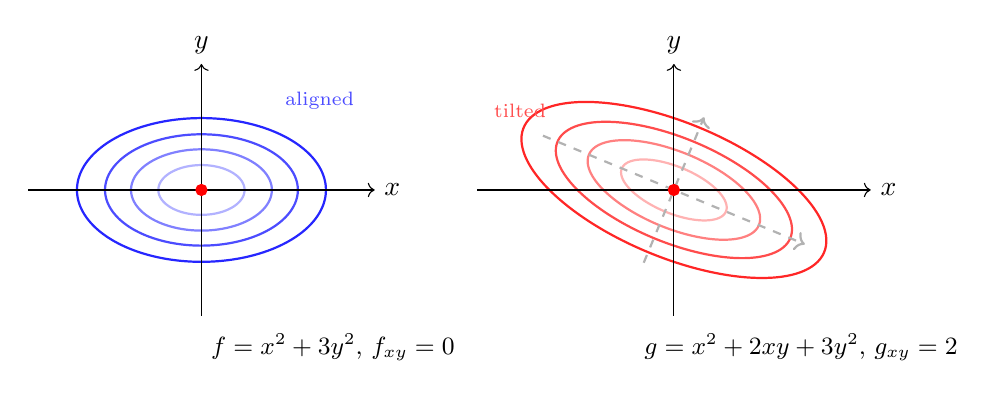
\begin{tikzpicture}[scale=1.0]

% LEFT: f = x^2 + 3y^2  (axis-aligned ellipses)
\begin{scope}[xshift=-4.5cm]
  \foreach \c/\col in {0.3/blue!30, 0.8/blue!50, 1.5/blue!70, 2.5/blue!85}{
    \draw[\col, thick]
      plot[domain=0:360, samples=100, smooth]
      ({sqrt(\c)*cos(\x)}, {sqrt(\c/3)*sin(\x)});
  }
  \draw[->] (-2.2,0) -- (2.2,0) node[right]{$x$};
  \draw[->] (0,-1.6) -- (0,1.6) node[above]{$y$};
  \filldraw[red] (0,0) circle (2pt);
  \node[below right, font=\small] at (0,-1.7)
    {$f = x^2+3y^2$, $f_{xy}=0$};
  \node[above, font=\scriptsize, blue!70] at (1.5,0.9)
    {aligned};
\end{scope}

% RIGHT: g = x^2 + 2xy + 3y^2  (tilted ellipses)
\begin{scope}[xshift=1.5cm]
  % level curve g = c is (x+y)^2 + 2y^2 = c
  % parametrise: x+y = sqrt(c)*cos(t), y*sqrt(2) = sqrt(c)*sin(t)
  % so y = sin(t)*sqrt(c/2), x = sqrt(c)*cos(t) - sin(t)*sqrt(c/2)
  \foreach \c/\col in {0.3/red!30, 0.8/red!50, 1.5/red!70, 2.5/red!85}{
    \draw[\col, thick]
      plot[domain=0:360, samples=120, smooth]
      ({sqrt(\c)*cos(\x) - sin(\x)*sqrt(\c/2)},
       {sin(\x)*sqrt(\c/2)});
  }
  \draw[->] (-2.5,0) -- (2.5,0) node[right]{$x$};
  \draw[->] (0,-1.6) -- (0,1.6) node[above]{$y$};
  % eigenvectors of H_g: eigenvalues 4 +/- 2*sqrt(2)
  % eigenvector for 4+2sqrt(2): (1, 1+sqrt(2)) ~ (0.383, 0.924)
  % eigenvector for 4-2sqrt(2): (1, 1-sqrt(2)) ~ (0.924, -0.383)
  \draw[gray!60, dashed, thick, ->]
    (-1.8*0.924, 1.8*0.383) -- (1.8*0.924, -1.8*0.383);
  \draw[gray!60, dashed, thick, ->]
    (-1.0*0.383, -1.0*0.924) -- (1.0*0.383, 1.0*0.924);
  \filldraw[red] (0,0) circle (2pt);
  \node[below right, font=\small] at (-0.5,-1.7)
    {$g = x^2+2xy+3y^2$, $g_{xy}=2$};
  \node[above left, font=\scriptsize, red!70] at (-1.5,0.8)
    {tilted};
\end{scope}

\end{tikzpicture}
\end{center}

For $f$ (left): the level curves are ellipses with semi-axes
aligned along the $x$- and $y$-directions.  The curvature in
$x$ does not interact with the curvature in $y$.

For $g$ (right): the level curves are tilted ellipses.  The
dashed lines show the eigenvectors of $H_g$, which are the
true axes of curvature — they do not coincide with the
coordinate axes.  The mixed partial $g_{xy} = 2$ is the
coefficient describing this tilt: how much the slope in $x$
changes when we move in $y$.

\subsubsection*{What $f_{xy} = 0$ means in words}

The mixed partial $f_{xy}(x_0, y_0)$ answers: if we increase
$y$ slightly from $y_0$, does the slope of $f$ in the
$x$-direction change?  If $f_{xy} = 0$ everywhere, the
answer is no: the $x$-profile of $f$ (a cross-section by
fixed $y$) has the same shape regardless of $y$.  The two
variables are \emph{curvature-independent}: knowing the
curvature structure in $x$ tells you nothing about how
$y$ enters.

Equivalently: the Hessian is diagonal iff there exists a
decomposition $f(x,y) = u(x) + v(y)$ (locally near the
stationary point, up to second order).

\subsubsection*{The Fisher information block-diagonal assumption}

In the BP model, the Fisher information matrix is
\[
  \mathcal{J}(\theta)
  = -E\!\left[\frac{\partial^2 l}{\partial\theta\,\partial\theta'}\right],
  \qquad \theta = (\alpha, \beta),
\]
and the block-diagonal assumption is $\mathcal{J}_{\alpha\beta} = 0$.

\begin{remark}[Is this an assumption or a theorem?]
For the specific BP log-likelihood it is a \emph{theorem}, not
an extra assumption.  We verified it earlier by direct
computation: the cross second derivative
$\partial^2 l/\partial\alpha_j\,\partial\beta_k$ contains
factors $u_t$ or $(u_t^2 - \sigma_t^2)$, whose expectation
under the model is zero.  So $\mathcal{J}_{\alpha\beta} = 0$
follows from $E[u_t] = 0$ and $E[u_t^2] = \sigma_t^2$.

In Rao's general framework (Section~6e.3), the block-diagonal
condition is stated as a \emph{hypothesis} on the model,
because Rao is not working with a specific parametric family.
For any particular model one must verify it.  BP do so
implicitly, and Rao provides the general theorem that, given
this condition, the LM statistic takes the simplified form
$\mathrm{LM} = \hat{d}_2'\hat{\mathcal{J}}_{22}^{-1}\hat{d}_2$.

Geometrically: $\mathcal{J}_{\alpha\beta} = 0$ means the
``likelihood bowl'' near the restricted MLE has axes aligned
with the $(\alpha,\beta)$ coordinate system.  Optimising over
$\beta$ for fixed $\alpha$ is decoupled from optimising over
$\alpha$ for fixed $\beta$.  It is precisely this decoupling
that allows the nuisance $\beta$ to be eliminated without
affecting the $\alpha$-part of the test statistic.
\end{remark}

%--------------------------------------------------------------------

\subsection{Rao's asymptotic score result: the theoretical basis for \texorpdfstring{$\chi^2$}{chi-squared}}
\label{subsec:rao-score}

\subsubsection*{Setup (Rao 1973, Section 6e.1)}

Let $x_1,\ldots,x_n$ be i.i.d.\ with density $p(x,\theta)$ and
$\theta = (\theta_1,\ldots,\theta_q)^\top \in \mathbb{R}^q$.  Define the
log-likelihood, score vector, and Fisher information:
\begin{align*}
  l(\theta) &= \sum_{i=1}^n \log p(x_i,\theta), \\
  V(\theta) &= \frac{\partial l}{\partial\theta}
  \quad \text{($q$-vector)}, \\
  F(\theta) &= -E\!\left[\frac{\partial^2 l}{\partial\theta\,
    \partial\theta'}\right]
  = n\,\mathcal{I}(\theta)
  \quad \text{($q\times q$ matrix)}.
\end{align*}
By the score identity: $E_\theta[V(\theta)] = 0$.  By the CLT
applied to i.i.d.\ score contributions:
\[
  \frac{1}{\sqrt{n}}\,V(\theta)
  \;\xrightarrow{d}\; \mathcal{N}(0,\, \mathcal{I}(\theta))
  \quad \text{as } n\to\infty.
\]

\subsubsection*{Simple hypothesis: $H_0:\theta = \theta_0$ (Section 6e.2)}

Rao proposes the \textbf{efficient score statistic}:
\[
  S_0 \;=\; V_0'\,F_0^{-1}\,V_0,
  \qquad V_0 = V(\theta_0),\quad F_0 = F(\theta_0).
\]
Under $H_0$: $V_0/\sqrt{n} \to \mathcal{N}(0,\mathcal{I})$, so
$V_0'\,F_0^{-1}\,V_0 \xrightarrow{d} \chi^2(q)$.

This is asymptotically equivalent to the likelihood-ratio statistic
$-2\log\Lambda$ and Wald's statistic $W_0$.  All three have the same
limiting $\chi^2(q)$ distribution under $H_0$ (proved by Rao via
Taylor expansion and the properties of efficient estimators).

The advantage of $S_0$: it does not require computing the MLE
$\hat\theta$ explicitly.  It only requires evaluating the
log-likelihood at $\theta_0$.

\subsubsection*{Composite hypothesis (Section 6e.3, pp. 418--419)}

Now the null is $H_0: R_j(\theta) = 0$ for $j = 1,\ldots,k$ ---
$k$ restrictions on $q$ parameters.  The free parameters under $H_0$
number $s = q - k$.

Let $\hat\theta$ be the unrestricted MLE and $\hat\theta^*$ the
\emph{restricted MLE} (constrained to $H_0$).  Rao's efficient score
test for the composite hypothesis (equation 6e.3.6) is:
\[
  S_* \;=\; V_*'\,F_*^{-1}\,V_*,
  \qquad V_* = V(\hat\theta^*),\quad F_* = F(\hat\theta^*).
\]

\begin{proposition}[Rao 1973, p.~419]
Under $H_0$ and regularity conditions, $S_* \xrightarrow{d} \chi^2(k)$.
All three statistics $S_*$, $W_*$, and $-2\log\Lambda_*$ are
asymptotically equivalent and have this limit.
\end{proposition}

\subsubsection*{Why the restricted MLE and not the unconstrained one}

\textbf{At the unconstrained MLE} $\hat\theta$: $V(\hat\theta) = 0$
by the first-order conditions of optimisation.  Therefore
$S_* = 0$ — identically zero and useless.

\textbf{At the restricted MLE} $\hat\theta^*$: the free parameters
$(\theta_3,\ldots,\theta_q)$ are at their optimum under the constraint,
so their score components are zero.  But the score in the constrained
directions $(\theta_1,\ldots,\theta_k)$ is generally non-zero and
measures how strongly the likelihood ``pushes'' against the constraint.
It is this non-zero part that constitutes the test.

\subsubsection*{Why the result is $\chi^2(k)$, not $\chi^2(q)$}

Under $H_0$, $\hat\theta^* \xrightarrow{p} \theta_0$ (the restricted
MLE is consistent for the true parameter).  So $V_* \approx V(\theta_0)$
for large $n$.

The score vector $V(\theta_0)$ is a $q$-dimensional random vector with
mean~$0$.  But $k$ of its coordinates are eliminated by the
first-order conditions at $\hat\theta^*$ (the unconstrained
directions have zero score).  Only the $k$ constrained coordinates
remain, and under the block-diagonal assumption these are
asymptotically $\mathcal{N}(0, F_{22})$ in $k$ dimensions.  The
quadratic form $V_*'F_*^{-1}V_*$ then equals approximately
$\chi^2(k)$.

Formally: Rao proves (p.~419) that $2[l(\hat\theta) - l(\hat\theta^*)]
\approx V_*'(F^{-1} - M H^{-1} M') V_*$ where $M$ is the matrix of
derivative of the constraints with respect to the free parameters,
and $H$ is their information matrix.  The idempotency of the
relevant matrix gives $\chi^2$ with degrees of freedom equal to
the rank of the idempotent, which is $k = q - s$.

\subsubsection*{Simple example: $\mathcal{N}(\mu,1)$, $H_0:\mu=0$}

$n$ observations, $\theta = \mu$, $q = 1$, $k = 1$.  The null is
simple.  $H_0$ constrains $\mu = 0$, leaving no free parameters.

\[
  l(\mu) = -\tfrac{n}{2}\log(2\pi) - \tfrac{1}{2}\sum(x_i-\mu)^2,
  \quad
  V = \sum(x_i-\mu), \quad F = n.
\]

Restricted MLE: $\hat\mu^* = 0$ (the only value satisfying $H_0$).

Score at restricted MLE: $V_* = \sum x_i = n\bar{x}$.

Rao statistic: $S_* = (n\bar x)^2/n = n\bar{x}^2$.

Under $H_0$: $\sqrt{n}\bar{x}\sim\mathcal{N}(0,1)$, so
$n\bar{x}^2\sim\chi^2(1)$. \checkmark  This is the squared $z$-test.

\subsubsection*{Example with nuisance: $\mathcal{N}(\mu,\sigma^2)$,
$H_0:\mu=0$, $\sigma^2$ unknown}

Now $\theta = (\mu,\sigma^2)$, $q=2$, $k=1$, $s=1$ ($\sigma^2$ free).

Restricted MLE: $\hat\mu^* = 0$,
$\hat\sigma^{*2} = n^{-1}\sum x_i^2$.

Score at $\hat\theta^*$:
\[
  V_\mu\big|_{\hat\theta^*}
  = \frac{\sum x_i}{\hat\sigma^{*2}} = \frac{n\bar x}{\hat\sigma^{*2}},
  \qquad
  V_{\sigma^2}\big|_{\hat\theta^*}
  = -\frac{n}{2\hat\sigma^{*2}} + \frac{\sum x_i^2}{2\hat\sigma^{*4}}
  = 0 \quad\checkmark
\]
(the $\sigma^2$-score is zero by the definition of $\hat\sigma^{*2}$).

Block-diagonal Fisher information for $\mathcal{N}(\mu,\sigma^2)$:
$\mathcal{J}_{\mu,\sigma^2} = 0$ (a standard calculation).  Therefore:
\[
  S_* \;=\; \hat{V}_\mu^2\,/\,F_{\mu\mu}
  \;=\; \frac{(n\bar x/\hat\sigma^{*2})^2}{n/\hat\sigma^{*2}}
  \;=\; \frac{n\bar x^2}{\hat\sigma^{*2}}
  \;\xrightarrow{d}\; \chi^2(1) \text{ under } H_0.
\]
The nuisance $\sigma^2$ entered only through $\hat\sigma^{*2}$
and dropped out cleanly, thanks to the block-diagonal structure
(§\,\ref{subsec:mixed-partials}).

\subsubsection*{Connection to BP}

BP set $\theta = (\alpha_0, \alpha_1,\ldots,\alpha_q, \beta_0,\beta_1,
\ldots,\beta_p)$ with $H_0: \alpha_1 = \cdots = \alpha_q = 0$.
The number of restrictions is $k = q$.  Restricted MLE =~OLS.
Block-diagonal Fisher information = verified from $E[u_t] = 0$.

Rao's theorem then gives: $S_* \xrightarrow{d} \chi^2(q)$ under $H_0$.
This is the theoretical basis for the $\chi^2(p-1)$ in BP's notation
(where $p = q+1$ includes the intercept in $\alpha$).

%--------------------------------------------------------------------

\subsection{The LM statistic: conditional score, restricted MLE, and block structure}
\label{subsec:lm-general}

We follow Boris's notes of July~18, 2026 (note~66).

\subsubsection*{What BP call ``the score''}

In the paper, BP differentiate the \emph{conditional} log-likelihood
$l(\theta) = \sum_i \log f_{Y|X}(y_i \mid x_i;\,\theta)$ with
respect to $\theta$ and call the result the score.  This is the
standard score vector:
\[
  d(\theta) \;=\; \frac{\partial\, l(\theta)}{\partial\theta}.
\]
BP refer to Rao (1973), \emph{Linear Statistical Inference and Its
Applications}, pp.~418--419, for the general Lagrange multiplier
framework.\footnote{Rao, C.\,R. (1973). \emph{Linear Statistical
Inference and Its Applications}, 2nd ed.\ Wiley.  A digitised copy:
\url{https://ia601508.us.archive.org/25/items/in.ernet.dli.2015.40834/2015.40834.Linear-Statistical-Inference-And-Its-Applications.pdf}.}
The Probabilist could not locate it freely online; Boris found both a paid
and a free version.  We will consult it later.

\subsubsection*{The general LM statistic}

From Rao (via BP): let $l(\theta)$ be the log-likelihood with
score $d = \partial l/\partial\theta$ and Fisher information
$\mathcal{J} = -E[\partial^2 l/\partial\theta\partial\theta']$.
The LM statistic for testing $H_0: \phi(\theta) = 0$ is
\[
  \mathrm{LM} \;=\; \hat{d}'\,\hat{\mathcal{J}}^{-1}\,\hat{d},
\]
where hats denote evaluation at $\hat\theta$ — the
\textbf{restricted} MLE satisfying $\phi(\hat\theta) = 0$.

\subsubsection*{The restricted MLE}

Boris emphasises: $\hat\theta$ is the argmax of the conditional
likelihood \emph{subject to the constraint} imposed by $H_0$, not
the unconstrained argmax.  In our concrete setting ($p = q = 1$):
\[
  \theta = (\alpha_0,\,\alpha_1,\,\beta_0,\,\beta_1) \in \mathbb{R}^4.
\]
The constraint is $\phi(\theta) = \alpha_1 = 0$.  The restricted MLE is
\[
  \hat\theta
  = \operatorname*{argmax}_{\alpha_0,\,\alpha_1=0,\,\beta_0,\,\beta_1}
    l(\alpha_0,\, 0,\, \beta_0,\, \beta_1),
\]
a three-dimensional optimisation.  One can show that $\hat\beta$
coincides with the OLS estimator and $\hat\alpha_0$ is determined
by $\hat\sigma^2 = n^{-1}\sum_i \hat{u}_i^2$.

\subsubsection*{How the score splits at $\hat\theta$}

Partition $\theta = (\alpha, \beta)$ and correspondingly
$d = (d_\alpha,\, d_\beta)^\top$.  At the restricted MLE,
the likelihood is stationary in the unconstrained directions $\beta$:
\[
  \hat{d}_\beta
  = \frac{\partial l}{\partial\beta}\bigg|_{\hat\theta} = 0.
\]
This is just the first-order condition: $\hat\theta$ is a genuine
interior optimum in $\beta$, so the gradient vanishes there.

The constrained direction $\alpha_1$ is fixed at zero by $H_0$, so
$\hat{d}_{\alpha_1}$ is generally \emph{non-zero} — it measures
how strongly the likelihood wants to move in the $\alpha_1$
direction, i.e.\ how much evidence there is against $H_0$.

Thus the score at $\hat\theta$ takes the form
\[
  \hat{d}
  = \begin{pmatrix} \hat{d}_{\alpha_0} \\[2pt]
    \hat{d}_{\alpha_1} \\[2pt] 0 \\[2pt] 0 \end{pmatrix},
\]
where the bottom two zeros are the $(\beta_0,\beta_1)$ components.

\subsubsection*{Block-diagonal assumption on $\mathcal{J}$}

BP additionally assume that the Fisher information matrix is
block-diagonal between $\alpha$ and $\beta$:
\[
  \mathcal{J}_{\alpha\beta}
  := -E\!\left[\frac{\partial^2 l}{\partial\alpha\,\partial\beta'}\right]
  = 0.
\]
Boris notes the distinction: $\hat{d}_\beta = 0$ is a consequence
of the first-order conditions (a fact about the optimum).  The
vanishing of $\mathcal{J}_{\alpha\beta}$ is an \emph{additional
assumption} that BP impose — and that we verified earlier by direct
computation: the cross-derivative has expectation zero because
$E[u_i] = 0$.

Under block-diagonality, the general LM statistic reduces to
\[
  \boxed{\mathrm{LM}
  \;=\; \hat{d}_\alpha'\,\hat{\mathcal{J}}_{\alpha\alpha}^{-1}\,
  \hat{d}_\alpha,}
\]
where only the $\alpha$-block appears.  The $\beta$-coordinates
are zero and contribute nothing.

\begin{remark}[What remains]
We have the general form.  The next subsection evaluates
$\hat{d}_\alpha$ and $\hat{\mathcal{J}}_{\alpha\alpha}$ for the
specific BP log-likelihood and shows the result equals
$\frac{1}{2}\,\widehat{\mathrm{ESS}}$ from the auxiliary
regression of $g_i = \hat{u}_i^2/\hat\sigma^2$ on $z_i$.
\end{remark}

%--------------------------------------------------------------------

\FloatBarrier
\subsection{The Breusch--Pagan test as a score test}
\label{subsec:bp-score}

We follow the Probabilist's notes of June~7, 2026.

\subsubsection*{Model hierarchy}

Simple regression with normally distributed errors:
\begin{align}
  y_i &= \beta_0 + \beta_1 x_i + \varepsilon_i, \qquad
  \varepsilon_i \sim \mathrm{ind}\; \mathcal{N}(0, \sigma_i^2),
  \tag{1} \\[4pt]
  \sigma_i^2 &= h(\alpha_0 + \alpha_1 z_i),
  \tag{2}
\end{align}
where $h(\cdot)$ is any twice-differentiable positive function, and
$z_i$ is an observable variable (often $z_i = x_i$, but not
necessarily).

Model~(1)\&(2) is a \emph{sub-model} of model~(1): it adds the
parametric constraint~(2) on how the variance moves. The null
hypothesis of homoscedasticity is
\[
  H_0: \alpha_1 = 0.
\]
Under $H_0$, equation~(2) gives $\sigma_i^2 = h(\alpha_0) =: \sigma^2$
for all $i$ — a constant.

\subsubsection*{The model-space picture}

\begin{figure}[ht]
\centering
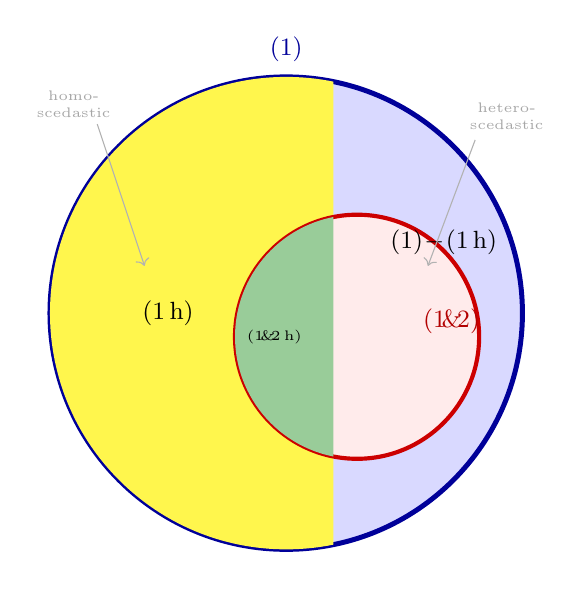
\begin{tikzpicture}[scale=1.0]
  % Large dark-blue circle: full model (1)
  \fill[blue!15] (0,0) circle (3.0cm);
  \draw[blue!60!black, line width=1.8pt] (0,0) circle (3.0cm);
  % Yellow homoscedastic region (1h): left crescent area
  \begin{scope}
    \clip (-3.2,-3.2) rectangle (0.6,3.2);
    \fill[yellow!70] (0,0) circle (3.0cm);
  \end{scope}
  % Sub-model circle (1&2): red contour, shifted right
  \fill[red!8] (0.9,-0.3) circle (1.55cm);
  \draw[red!80!black, line width=1.5pt] (0.9,-0.3) circle (1.55cm);
  % Green homoscedastic sub-model region (1&2 h): overlap of sub-model and yellow region
  \begin{scope}
    \clip (-3.2,-3.2) rectangle (0.6,3.2);
    \fill[green!50!black!40] (0.9,-0.3) circle (1.55cm);
  \end{scope}
  % Labels
  \node[font=\small\bfseries, blue!60!black] at (0, 3.35) {$(1)$};
  \node[font=\small, black] at (-1.5, 0.0) {$(1\,\mathrm{h})$};
  \node[font=\small, black] at (2.0, 0.9) {$(1)\!-\!(1\,\mathrm{h})$};
  \node[font=\small, red!70!black] at (2.1,-0.1) {$(1\!\&\!2)$};
  \node[font=\tiny, black] at (-0.15,-0.3) {$(1\!\&\!2\,\mathrm{h})$};
  % Arrow annotations
  \draw[->, gray!60, thin] (-2.4,2.4) -- (-1.8,0.6);
  \node[font=\tiny, gray!70, align=center] at (-2.7,2.65) {homo-\\scedastic};
  \draw[->, gray!60, thin] (2.4,2.2) -- (1.8,0.6);
  \node[font=\tiny, gray!70, align=center] at (2.8,2.5) {hetero-\\scedastic};
\end{tikzpicture}
\caption{The Probabilist's diagram (June~7, 2026).  The large dark-blue circle
is the full model~(1) — simple regression with unrestricted
heteroscedasticity.  It splits into the yellow region
$(1\,\mathrm{h})$ (homoscedastic) and the white region
$(1)-(1\,\mathrm{h})$ (heteroscedastic).  The smaller red-contour
circle $(1\&2)$ is the sub-model that additionally imposes the
parametric form~(2) on the variance; it splits into the green region
$(1\&2\,\mathrm{h})$ (homoscedastic sub-model) and its local
complement.  We want to test white against yellow, but instead test
blue against yellow — the difference is parametrised by $\alpha_1=0$
or not.}
\label{fig:bp-circles}
\end{figure}

The ideal test would compare the heteroscedastic part of model~(1)
(white) against the homoscedastic part (yellow).  We cannot do this
directly — the white region has no finite-dimensional parametrisation.
Instead, the BP test embeds the problem into the parametric
sub-model~(1)\&(2) and tests the green region against the yellow one,
i.e.\ $\alpha_1 = 0$ inside~(2).

Note the Probabilist's point: the $z_i$ are \emph{specific} and must be
observable.  The authors kept $z_i$ general (rather than always
setting $z_i = x_i$) to nest heteroscedastic models from earlier
literature.

\subsubsection*{Why the score test}

The score (LM) test is ideally suited here.  Under $H_0$ the
restricted MLE is just OLS — no iterative optimisation needed.  The
test asks: does the log-likelihood \emph{want to move} away from the
null, i.e.\ is its slope with respect to $\alpha_1$ large at the OLS
solution?

\subsubsection*{Log-likelihood and score}

The log-likelihood for model~(1)\&(2) is
\[
  \ell(\beta,\alpha)
  = \mathrm{const}
    - \tfrac{1}{2}\sum_i \log\sigma_i^2
    - \tfrac{1}{2}\sum_i \frac{\varepsilon_i^2}{\sigma_i^2},
  \qquad \sigma_i^2 = h(\alpha_0 + \alpha_1 z_i).
\]
Differentiating with respect to $\alpha_1$ and evaluating at
$H_0$ (where $\sigma_i^2 = \hat\sigma^2$ and $\varepsilon_i =
\hat{u}_i$):
\[
  \left.\frac{\partial\ell}{\partial\alpha_1}\right|_{H_0}
  = \frac{h'(\hat\alpha_0)}{2\hat\sigma^2}
    \sum_i \left(\frac{\hat{u}_i^2}{\hat\sigma^2} - 1\right) z_i.
\]
Define $g_i := \hat\sigma^{-2}\hat{u}_i^2$ and $f_i := g_i - 1$.
The score is proportional to $\sum_i f_i z_i$ — the
sample covariance between the normalised squared residuals and $z_i$.

\subsubsection*{Fisher information and the cancellation of $h'$}

The $({\alpha_1},{\alpha_1})$ block of the Fisher information,
evaluated at $H_0$, is
\[
  \mathcal{J}_{\alpha_1\alpha_1}\big|_{H_0}
  = \frac{[h'(\hat\alpha_0)]^2}{2\hat\sigma^4}\sum_i z_i^2.
\]
The LM statistic $\hat{d}'\hat{\mathcal{J}}^{-1}\hat{d}$ therefore
equals
\[
  LM
  = \frac{\bigl(\sum_i f_i z_i\bigr)^2}{\sum_i z_i^2},
\]
where the factor $h'(\hat\alpha_0)$ has \emph{cancelled completely}.
The statistic does not depend on the choice of $h$ — only on the
residuals $\hat{u}_i$ and the variable $z_i$.

\subsubsection*{Connection to the auxiliary regression}

Write $z_i = (1, z_i)'$ for the general case with a constant in~(2).
Breusch and Pagan show (by the algebra $f = g - \iota$, $\iota'g = N$,
$f'Z(Z'Z)^{-1}Z'\iota = 0$) that the LM statistic equals one half
the explained sum of squares in the regression of $g_i$ on $z_i$:
\[
  LM = \tfrac{1}{2}\,\mathrm{ESS}(g_i \sim z_i)
  \;\xrightarrow{d}\; \chi^2_{p-1}
  \quad\text{under }H_0,
\]
where $p-1$ is the number of variance regressors (excluding the
constant $\alpha_0$).  For simple regression with $z_i = x_i$ this
gives $\chi^2_1$.

The practical formula $nR^2 \sim \chi^2_1$ follows because
$\mathrm{ESS} = R^2 \cdot \mathrm{TSS}$ and $\mathrm{TSS}$ of $g_i$
equals $2n$ asymptotically under normality (since $g_i =
\hat\sigma^{-2}\hat{u}_i^2 \approx \chi^2_1$ and $\mathrm{Var}(\chi^2_1)
= 2$).

\medskip\noindent
\textbf{Remark (finite samples).}
The $\chi^2$ approximation can be poor for small $n$.
Breusch and Pagan's own simulations (Table~I of the paper) show that
at $n=20$ the actual Type~I error at a nominal 5\% level is closer to
1--2\%, so conservative critical values are advisable.
The Koenker (``studentised'') variant drops the normality assumption
and is better calibrated in small samples.

%--------------------------------------------------------------------




\end{document}
